\documentclass[10pt,preprint,blind,clearpagebib]{sigplanconf}

\usepackage{listings}
\usepackage{enumitem}
\usepackage[hyphens]{url}
\usepackage[svgnames]{xcolor}
\definecolor{lcl}{RGB}{140,0,100}
\usepackage[colorlinks=true,breaklinks,draft=false]{hyperref}
\hypersetup{urlcolor=lcl,linkcolor=lcl,citecolor=lcl}
\newcommand{\doi}[1]{doi:~\href{http://dx.doi.org/#1}{\Hurl{#1}}}
\usepackage{amssymb}
\usepackage{multicol}
\usepackage{xcolor}
\usepackage{graphicx}
\usepackage[fleqn]{amsmath}
\usepackage{graphics} 
\usepackage{stmaryrd}
\usepackage{amsthm}
\usepackage{ftnright}
\usepackage[T1]{fontenc}
\usepackage{semantic}
\usepackage{enumitem}
\usepackage[hang,flushmargin]{footmisc} 
\usepackage[notquote]{hanging}
\usepackage{flushend}

% =================================================================================================

% TODO: Discuss 'stability' of the inference (minor change in schema does not cause dramatic cahnges)
% TODO: Say that variant is a last-resort thing
% TODO: Practical evaluation (lots of downloads, lots of Github - how often people customize samples?)
% TODO: Explain why we need option type (because T + null is a variant)
% TODO: In the PLDI version, we delete all the unnecessary runtime conversions
% but we should say that those happen for practical reasons (e.g. float -> int, or anyhing to string)

\urlstyle{sf}

\makeatletter
\renewcommand{\@makefntext}[1]{%
  \parindent 1em%
  \raggedright
  \begin{hangparas}{0.8em}{1}
  \noindent {$^{\@thefnmark}$~#1}
  \end{hangparas}
}
\makeatother

\newcommand{\langl}{\begin{picture}(4.5,7)
\put(1.1,2.5){\rotatebox{60}{\line(1,0){5.5}}}
\put(1.1,2.5){\rotatebox{300}{\line(1,0){5.5}}}
\end{picture}}
\newcommand{\rangl}{\begin{picture}(4.5,7)
\put(.9,2.5){\rotatebox{120}{\line(1,0){5.5}}}
\put(.9,2.5){\rotatebox{240}{\line(1,0){5.5}}}
\end{picture}}

\newcommand{\lang}{\begin{picture}(5,7)
\put(1.1,2.5){\rotatebox{45}{\line(1,0){6.0}}}
\put(1.1,2.5){\rotatebox{315}{\line(1,0){6.0}}}
\end{picture}}
\newcommand{\rang}{\begin{picture}(5,7)
\put(.1,2.5){\rotatebox{135}{\line(1,0){6.0}}}
\put(.1,2.5){\rotatebox{225}{\line(1,0){6.0}}}
\end{picture}} 

\newcommand{\llangl}{\langl\hspace{-0.35em}\langl}
\newcommand{\rrangl}{\rangl\hspace{-0.35em}\rangl}

\definecolor{cmtclr}{rgb}{0.0,0.6,0.0}
\definecolor{numclr}{rgb}{0.0,0.4,0.0}
\definecolor{kvdclr}{rgb}{0.0,0.0,0.6}
\definecolor{strclr}{rgb}{0.5,0.1,0.0}
\definecolor{prepclr}{rgb}{0.0,0.0,0.0}

\newcommand{\kvd}[1]{\textnormal{\textcolor{kvdclr}{\sffamily #1}}}
\newcommand{\num}[1]{\textnormal{\textcolor{numclr}{\sffamily #1}}}
\newcommand{\str}[1]{\textnormal{\textcolor{strclr}{\sffamily "#1"}}}
\newcommand{\strf}[1]{\textnormal{\textcolor{strclr}{\sffamily #1}}}
\newcommand{\ident}[1]{\textnormal{\sffamily #1}}
\newcommand{\lident}[1]{\textnormal{\sffamily\`{}\hspace{-0.25em}\`{}\hspace{-0.1em}#1\`{}\hspace{-0.25em}\`{}}}
\newcommand{\cmt}[1]{\textit{\sffamily\textcolor{cmtclr}{#1}}}

\newcommand{\lsep}[0]{\;\; | \;\;}
\newcommand{\narrow}[1]{\hspace{-0.7em} #1 \hspace{-0.7em}}

\newcommand{\tsep}[0]{\; \triangledown \;}
\newcommand{\tytag}{\ident{tag}}
\newcommand{\dropopt}[1]{\lfloor#1\rfloor}
\newcommand{\addopt}[1]{\lceil#1\rceil}
\newcommand{\tytagof}{\ident{tagof}}
\newcommand{\nameoftag}{\ident{nameof}}

\newcommand{\reduce}{\rightsquigarrow}

\newcommand{\sem}[1]{\llbracket #1 \rrbracket}
\newcommand{\semalt}[1]{\llangl #1 \rrangl}

\newtheorem{definition}{Definition}
\newtheorem{theorem}{Theorem}
\newtheorem{corollary}[theorem]{Corollary}
\newtheorem{lemma}[theorem]{Lemma}

% =================================================================================================

\begin{document}

\special{papersize=8.5in,11in}
\setlength{\pdfpageheight}{\paperheight}
\setlength{\pdfpagewidth}{\paperwidth}
\conferenceinfo{CONF 'yy}{Month d--d, 20yy, City, ST, Country} 
\copyrightyear{20yy} 
\copyrightdata{978-1-nnnn-nnnn-n/yy/mm} 
%\doi{nnnnnnn.nnnnnnn}

%\titlebanner{Unpublished draft, March 2015}        % These are ignored unless
%\preprintfooter{short description of paper}        % 'preprint' option specified.

\title{Types From Data: \textnormal{Making structured schema-free data formats first-class citizens in F\#}}
%\subtitle{Subtitle Text, if any}

\authorinfo{Tomas Petricek}
           {University of Cambridge}
           {tomas@tomasp.net}
\authorinfo{Gustavo Guerra}
           {Microsoft Corporation, London}
           {gustavo@codebeside.org}
\authorinfo{Don Syme}
           {Microsoft Research, Cambridge}
           {dsyme@microsoft.com}
\maketitle

% =================================================================================================

\begin{abstract}
Most modern applications interact with external services and access data in structured formats such 
as XML, JSON and CSV. Static type systems do not understand such formats making accessing data more 
cumbersome. Should we give up and leave the messy world of external data to dynamic typing and 
runtime checks? Of course, not!

We show how to integrate external data sources into the F\# type system. As most real-world data
does not come with an explicit schema, we develop a type inference algorithm that infers a type from 
representative sample documents and integrate it into the F\# type system using type providers.

Our library significantly reduces the amount of code that developers need to write when 
accessing and producing data. It also provides additional safety guarantees when contrasted 
with the weakly typed techniques used to anually project data to and from explicit type definitions.
\end{abstract}

\category{D.3.3}{Programming Languages}{Language Constructs and Features }
\keywords F\#, Type Providers, Inference, JSON, XML



% =================================================================================================
%
%   ###                                                                       
%    #  #    # ##### #####   ####  #####  #    #  ####  ##### #  ####  #    # 
%    #  ##   #   #   #    # #    # #    # #    # #    #   #   # #    # ##   # 
%    #  # #  #   #   #    # #    # #    # #    # #        #   # #    # # #  # 
%    #  #  # #   #   #####  #    # #    # #    # #        #   # #    # #  # # 
%    #  #   ##   #   #   #  #    # #    # #    # #    #   #   # #    # #   ## 
%   ### #    #   #   #    #  ####  #####   ####   ####    #   #  ####  #    # 
%
% =================================================================================================

\section{Introduction}
\label{sec:introduction}

Applications for taking notes, searching train schedules or finding tomorrow's weather all 
communicate with one or more services over the network and present the aggregated data. 
Increasing number of such services provide REST-based end-points that return data as CSV, XML
or JSON. Despite numerous schematization efforts, most services do not come with an 
explicit schema. At best, the documentation provides sample responses for typical requests.
These samples seem to be the best, or at least most widespread, way we have collectively found to 
characterize most information transfer in the world today.

For example, openweathermap.org provides an end-point for getting the current weather for a 
given city\footnote{See ``Current weather data'': \url{http://openweathermap.org/current}}. 
The documentation describes the URL parameters and shows one sample JSON to illustrate the typical
response structure. Using a standard library for working with JSON and HTTP, we might call the 
service and read the temperature as follows:
%
\begin{equation*}
\begin{array}{l}
 \kvd{let}~\ident{doc}=\ident{Http.Request}(\str{http://api.owm.org/?q=NYC}) \\
 \kvd{match}~\ident{JsonValue.Parse}(\ident{doc})~\kvd{with} \\
 |~\ident{Record}(\ident{root})\rightarrow \\
 \quad \kvd{match}~\ident{Map.find}~\str{main}~\ident{root}~\kvd{with} \\
 \quad |~\ident{Record}(\ident{main})\rightarrow \\
 \quad \quad \kvd{match}~\ident{Map.find}~\str{temp}~\ident{main}~\kvd{with} \\
 \quad \quad |~\ident{Number}(\ident{num})\rightarrow \ident{printfn}~\str{Nice \%f degrees!}~\ident{num} \\
 \quad \quad |~\_\rightarrow \ident{failwith}~\str{Incorrect format} \\
 \quad |~\_\rightarrow \ident{failwith}~\str{Incorrect format} \\
 |~\_\rightarrow \ident{failwith}~\str{Incorrect format} 
\end{array}
\end{equation*}
%
The code assumes that the response has a particular format described in the documentation. The
root node must be a record with a \str{main} field, which has to be another record containing
a numerical \str{temp} field. When the format is incorrect, the data access simply fails
with an exception. The code, while not immediately unsound, is manifestly prone to errors if
strings are mispelled.

Using the JSON type provider from F\# Data, we can write code with exactly the 
same functionality in two lines:
%
\begin{equation*}
\begin{array}{l}
 \kvd{type}~\ident{W} = \ident{JsonProvider}\langl\str{http://api.owm.org/?q=NYC}\rangl \\[0.1em]
 \ident{printfn}~\str{Nice \%f degrees!}~(\ident{W.GetSample().Main.Temp})
\end{array}
\end{equation*}
%
$\ident{JsonProvider}\langl\str{...}\rangl$ invokes a type provider at 
compile-time with the URL as a sample. The type provider infers the structure of the response
and provides a type with a \ident{GetSample} method that returns a parsed JSON with nested
properties \ident{Main.Temp}, returning the temperature as a number. 

In short, \emph{the types come from the sample data}.  From our experience, 
this technique is both immensely practical and surprisingly effective in achieving sound 
information interchange in heterogeneous systems.
The rest of the paper describes the mechanism and discusses its safety properties. 
The key novel contributions are:

\begin{itemize}
\item We present F\# Data type providers for XML, CSV and JSON (\S\ref{sec:providers}) 
  and practical aspects of their implementation that contributed to their industrial 
  adoption (\S\ref{sec:impl}). 

\item We describe a predictable type inference algorithm for structured data formats that
  underlies the type providers (\S\ref{sec:inference}) based on a \emph{common supertype}
  relation.

\item We give a formal model (\S\ref{sec:formal}) and use it to prove
  \emph{relativized type safety} for the type providers (\S\ref{sec:safety}).
  This adapts the ML-style type safety for the context of the web.
\end{itemize}



% =================================================================================================
%
%   #######                                                                                  
%      #    #   # #####  ######    #####  #####   ####  #    # # #####  ###### #####   ####  
%      #     # #  #    # #         #    # #    # #    # #    # # #    # #      #    # #      
%      #      #   #    # #####     #    # #    # #    # #    # # #    # #####  #    #  ####  
%      #      #   #####  #         #####  #####  #    # #    # # #    # #      #####       # 
%      #      #   #      #         #      #   #  #    #  #  #  # #    # #      #   #  #    # 
%      #      #   #      ######    #      #    #  ####    ##   # #####  ###### #    #  ####  
%
% =================================================================================================

\section{Type providers for structured data formats}
\label{sec:providers}

We start with an informal overview that shows how F\# Data type providers simplify working with 
JSON, XML and CSV. We introduce the necessary aspects of F\# type providers along the 
way. The examples in this section illustrate a number of key design principles of the type inference 
algorithm:

\begin{itemize}
\item The mechanism is predictable. The user directly works with the inferred types and should 
  understand why a specific type was inferred from a given sample\footnote{In particular, we do 
  not use probabilistic methods where adding additional sample could change the shape of the type.}.

\item The inference mechanism prefers types with properties (records). This is to allow extensible (open-world)
  data formats, as we will explain. It also interacts well with developer tooling --
  most editors provide code completion hints on ``.'' and so types with properties (records)
  are easier to use than typessuch as discriminated unions that require pattern matching.

\item Finally, the mechanism handles a number of practical concerns important in the real world. This includes 
  support for different numerical types, \kvd{null} values and missing data.
\end{itemize}

% --------------------------------------------------------------------------------------------------

\subsection{Working with JSON documents}
\label{sec:providers-json}

The JSON format used in \S\ref{sec:introduction} is a popular data exchange format based on 
JavaScript data structures. The following is the definition of \ident{JsonValue} 
used earlier to represent JSON:
%
\begin{equation*}
\begin{array}{l}
 \kvd{type}~\ident{JsonValue} = \\[0.1em]
 \quad|~ \ident{Number}~\kvd{of}~\ident{decimal} ~~|~ \ident{Null} \\[0.1em]
 \quad|~ \ident{String}~\kvd{of}~\ident{string} \qquad\, |~ \ident{Boolean}~\kvd{of}~\ident{bool} \\[0.1em]
 \quad|~ \ident{Record}~\kvd{of}~\ident{Map}\langl\ident{string}, \ident{JsonValue}\rangl \\[0.1em]
 \quad|~ \ident{Array}~\kvd{of}~\ident{JsonValue}[] \\[0.1em]
\end{array}
\end{equation*}
%
The earlier example used only a nested record containing a number. To demonstrate other 
aspects of the JSON type provider, we look at an example that also involves an array:
%
{\small{
\begin{verbatim}
  [ { "name":"Jan", "age":25 }, { "name":"Tomas" },
    { "name":"Alexander", "age":3.5 } ]
\end{verbatim}
}}
%
\noindent
Say we want to print the names with an age if it is available. The standard approach would 
be to pattern match on the parsed \ident{JsonValue}, check that the top-level node is a \ident{Array}
and iterate over the elements checking that each is a \ident{Record} with certain properties. We
would throw an exception or skip values in an incorrect format. Even if we defined helper functions, 
we would still need to specify field names as strings, which is error prone and can not be 
statically checked.

Assuming \strf{people.json} is the above example and \ident{data} is a string containing
JSON in the same format, we can write:
%
\begin{equation*}
\begin{array}{l}
 \kvd{type}~\ident{People}~=~\ident{JsonProvider}\langl\str{people.json}\rangl\hspace{1em} \\[0.6em]
 \kvd{for}~\ident{item}~\kvd{in}~\ident{People.Parse}(\ident{data})~\kvd{do}\\[0.1em]
 \quad\ident{printf}~\str{\%s }~\ident{item.Name}\\[0.1em]
 \quad\ident{Option.iter}~(\ident{printf}~\str{(\%f)})~\ident{item.Age}
\end{array}
\end{equation*}
%
The code achieves a similar simplicity as when using dynamically typed languages, but is statically 
type-checked. In contrast to the earlier example, we now use a local file \strf{people.json} as a 
sample for the type inference, but then processes data from another source, which must conform to the
schema types implied by the sample.

\paragraph{Type providers.}
The notation $\ident{JsonProvider}\langl\str{people.json}\rangl$ passes a \emph{static parameter} 
to the type provider. Static parameters are resolved at compile-time and have to be constant. 
The provider analyzes the sample and generates a type that we name \ident{People}. In most F\# 
editors, the type provider is also executed at development-time and the provided types are 
used in auto-completion and checking.

The \ident{JsonProvider} uses a type inference algorithm (\S\ref{sec:inference})  and
infers the following types from the sample:
%
\begin{equation*}
\begin{array}{l}
 \kvd{type}~\ident{Entity}~=  \\
 \quad \kvd{member}~\ident{Name}~:~\ident{string} \\
 \quad \kvd{member}~\ident{Age}~:~\ident{option}\langl \ident{decimal}\rangl \\[0.5em]
 \kvd{type}~\ident{People}~=  \\
 \quad \kvd{member}~\ident{GetSample}~:~\ident{unit}~\rightarrow~\ident{Entity}[] \\
 \quad \kvd{member}~\ident{Parse}~:~\ident{string}~\rightarrow~\ident{Entity}[] \\
\end{array}
\end{equation*}
%
The type \ident{Entity} represents the person. The field \ident{Name} is available for all
sample values and is inferred as \ident{string}. The field \ident{Age} is marked as optional,
because the value is missing in one sample. The two sample ages are an integer $25$ and a 
decimal $3.5$ and so the common inferred type is \ident{decimal}.

The type \ident{People} has two methods for reading data. \ident{GetSample} parses the
sample used for the inference and \ident{Parse} parses a JSON string containing data in the same 
format as the sample. Both methods return an array of \ident{Entity} values.

\paragraph{Error handling.}
In addition to the structure of the types, the type provider also specifies what code should be 
executed at run-time in place of \ident{item.Name} and other operations. The runtime behaviour is 
the same as in the earlier hand-written sample (\S\ref{sec:introduction}). A member access 
throws an exception if the document does not have the expected format.

Informally, the safety property (\S\ref{sec:safety}) states that if the inputs
are subtypes of some of the provided samples (i.e.~the samples are representative), then
no exceptions will occur. In other words, we cannot avoid all failures, but we can prevent some.
If OpenWeatherMap changes the response format, the sample in \S\ref{sec:introduction}
will not re-compile and the user knows that the code needs to be changed. What this means for
type safety is discussed in \S\ref{sec:safety-discuss}.

\paragraph{The role of records.}
The sample code is easy to write thanks to the fact that most F\# editors provide code completion
when ``.'' is typed. The developer does not need to look at the sample JSON file to see what fields
are available for a person. To support this scenario, our inference algorithm prefers records 
(we also treat XML elements and CSV rows as records) and only infers types that require pattern 
matching as the last resort.

In the above example, this is demonstrated by the fact that \ident{Age} is marked as optional.
An alternative is to provide two different record types (one with \ident{Name} and other with 
\ident{Name} and \ident{Age}), but this would complicate the processing code.

% -------------------------------------------------------------------------------------------------

\subsection{Processing XML documents}
\label{sec:providers-xml}

XML documents are formed by nested elements with attributes. We can view elements as records with 
a field for each attribute and an additional special field for the nested contents (which is a 
collection of elements).

Consider a simple extensible document format where a root element
{\ttfamily\small <doc>} can contain a number of document elements, one of which is
{\ttfamily\small <heading>} representing headings:
%
{\small{
\begin{verbatim}
  <doc>
    <heading>Working with JSON</heading>
    <p>Type providers make this easy.</p>
    <heading>Working with XML</heading>
    <p>Processing XML is as easy as JSON.</p>
    <image source="xml.png" />
  </doc>
\end{verbatim}
}}
%
\noindent
The F\# Data library has been designed primarily to simplify reading data. For example,
say we want to print all headings in the document. The sample shows a part of the document structure 
(in particular the {\ttfamily\small <heading>} element), but it does not show all possible elements 
(say, {\ttfamily\small <table>}). Assuming the above document is \strf{sample.doc}, we can write:
%
\noindent
\begin{equation*}
\begin{array}{l}
 \kvd{type}~\ident{Document}~=~\ident{XmlProvider}\langl\str{sample.doc}\rangl\hspace{1em} \\[0.5em]
 \kvd{let}~\ident{root}~=~\ident{Document.Load}(\str{http://.../another.doc})\\
 \kvd{for}~\ident{elem}~\kvd{in}~\ident{root.Doc}~\kvd{do}\\
 \quad\kvd{match}~\ident{elem.Heading}~\kvd{with} \\
 \quad|~\ident{Some text} \rightarrow \ident{printf}~\str{ - \%s }~\ident{text}\\
 \quad|~\ident{None} \rightarrow ()\\
\end{array}
\end{equation*}
%
The example iterates over a collection of elements \ident{elem} returned by \ident{root.Doc}. 
The type provides a typed access to elements known from the sample document and so we can
write \ident{elem.Heading}, which returns an optional value.

\paragraph{Open world}

In the above example, we do not infer an F\# discriminated union type representing a choice between 
heading, paragraph and image. By its nature, XML is extensible and the sample cannot include all 
possible nodes\footnote{Even when the document structure is defined using XML Schema, documents may 
contain elements prefixed with other namespaces.}. 
The type is not closed -- the data might be some other element about which nothing is known.
This is the \emph{open-world assumption}. Supporting the open-world assumption is crucial when reading data from 
external data sources, because the sample document need only
mention possibilities relevant to the application. 

In the subsequent formalism, the type of \ident{elem} will initially be a top type 
annotated with the statically known possibilities (heading, paragraph, image). 
We call this a \emph{variant-annotated top type}.
However, variant-annotated top types are then removed in favour of record types
that have additional optional fields and the type inference minimzes the number of 
variant-annotated top types that appear in the resulting type --
a variant is not used if there is an alternative (Corollary~\ref{thm:no-unions}).

In this case, the variant-annotated top type is ultimately presented as the following F\# type:
%
\begin{equation*}
\begin{array}{l}
 \kvd{type}~\ident{Element}~=  \\[0.1em]
 \quad \kvd{member}~\ident{Heading}~:~\ident{option}\langl \ident{string} \rangl\\
 \quad \kvd{member}~\ident{Paragraph}~:~\ident{option}\langl \ident{string} \rangl\\
 \quad \kvd{member}~\ident{Image}~:~\ident{option}\langl \ident{Image} \rangl\\
\end{array}
\end{equation*}
%
This still provides access to the possible elements known statically from the sample.
The access is, however, deliberately weak, because the user needs to explicitly handle the casse when the value is none 
of the statically known elements. 
For example, the above code for  \strf{sample.doc} includes a \kvd{None -> ()} case to ensure that it will work 
correctly on a document containing elements not listed in the sample. Furthermore, 
the programmer is not \emph{forced} to consider each of the possiblities in the annotations. For example,
the program is not forced to include cases for  \ident{Paragraph} and \ident{Image}.  
Both of these weakenings are consistent with our design principles, 
which prefer records (with optional properties) over discriminated unions, in order to support 
open-world data and dot-driven developer tooling.

% Nothing forces the programmer to consider the cases

%The type is also not exclusive: it doesn't promise that only one of the cases returns a non-\ident{None} value.  

% -------------------------------------------------------------------------------------------------

\subsection{Summary}
In addition to JSON and XML (\S\ref{sec:providers-json}, \S\ref{sec:providers-xml}), F\# Data also 
implements a type provider for CSV. We treat CSV data as lists of records (with field for each 
column) and so handling of CSV is just a special case of our inference algorithm.

Throughout the introduction, we used data sets that demonstrate the typical issues that are frequent
in real-world inputs: \emph{missing data}, \emph{inconsistent encoding} of primitive values and 
\emph{heterogeneous structures}. The following JSON response with 
government debt information returned by the World Bank API\footnote{Available at 
\url{http://data.worldbank.org}} demonstrates all three problems:
%
{\small{
\begin{verbatim}
  [ { "page": 1, "pages": 5 },
    [ { "indicator": "GC.DOD.TOTL.GD.ZS",
        "date": "2012", "value": null },
      { "indicator": "GC.DOD.TOTL.GD.ZS",
        "date": "2010", "value": "35.14229" } ] ]
\end{verbatim}
}}
%
\noindent
First of all, the top-level element is a collection containing two values of different kind.
The first is a record with meta-data about the current page and the second is an array with data. 
The actual implementation supports a concept of heterogeneous collections (omitted in this paper
for space reasons) and provides a type with properties \ident{Record} for the former and 
\ident{Array} for the latter. Second, the \ident{value} is \kvd{null} for some records. Third, 
numbers can be represented in JSON as numeric literals (without quotes), but here, they are 
returned as string literals instead\footnote{This is often used to avoid non-standard numerical 
types of JavaScript.}.



% =================================================================================================
%
%   #######                                                                                  
%      #    #   # #####  ######    # #    # ###### ###### #####  ###### #    #  ####  ###### 
%      #     # #  #    # #         # ##   # #      #      #    # #      ##   # #    # #      
%      #      #   #    # #####     # # #  # #####  #####  #    # #####  # #  # #      #####  
%      #      #   #####  #         # #  # # #      #      #####  #      #  # # #      #      
%      #      #   #      #         # #   ## #      #      #   #  #      #   ## #    # #      
%      #      #   #      ######    # #    # #      ###### #    # ###### #    #  ####  ###### 
%
% =================================================================================================

\section{Type inference for structured data formats}
\label{sec:inference}

The type inference algorithm for structured formats is based on a subtyping relation. When 
inferring the type, we infer the most specific types of individual values (CSV rows, JSON or XML 
nodes) and recursively find a common supertype of all child nodes or all sample documents.

We first define the type of structured data $\sigma$. Note that this type is distinct 
from the programming language types $\tau$ (type providers generate the latter from the former). 
Next, we define the subtyping relation on structural types $\sigma$ and describe the algorithm 
for finding a common supertype. 

\subsection{Structural types}
\label{sec:inference-types}

We distinguish between \emph{non-nullable types} that always have a valid value (written as 
$\hat{\sigma}$) and \emph{nullable types} that encompass missing and \kvd{null} values 
(written as $\sigma$). We write $\nu$ for record field names and $\nu_?$ for names that can be empty:

\noindent
\begin{equation*}
\begin{array}{rcl}
 \hat{\sigma} &\narrow{=}& \nu_?\; \{ \nu_1 : \sigma_1, \ldots, \nu_n : \sigma_n \} \\[0.1em]
                &\narrow{|}& \ident{float} \lsep \ident{decimal} \lsep \ident{int} \lsep \ident{bool} \lsep \ident{string} 
 \\[0.6em] 
       \sigma &\narrow{=}& ~\hat{\sigma}~ \lsep \kvd{option}\langl \hat{\sigma} \rangl \lsep [\sigma] \\[0.1em]
              &\narrow{|}& \kvd{any}\langl\sigma_1, \ldots, \sigma_n\rangl \lsep ~\bot~ \lsep \kvd{null}
\end{array}
\end{equation*}
%
Non-nullable types include records (consisting of an optional name and fields with their types) 
and primitive types. Records arising from XML documents are named, while records used by 
JSON and CSV providers are unnamed. 

The three numerical types, \ident{int} for integers, \ident{decimal} for small precise decimal 
numbers and \ident{float} for floating-point numbers, are related by sub-typing as discussed in 
\S\ref{sec:inference-subtyping}.

Any non-nullable type can be wrapped in the \kvd{option} constructor to explicitly permit the 
\kvd{null} value. Type providers map \kvd{option} to the standard F\# option type. A collection $[\sigma]$ 
is also nullable and missing values or \kvd{null} are treated as empty collections. The type 
$\kvd{null}$ is inhabited by the $\kvd{null}$ value (using an overloaded notation) and $\bot$ 
is the bottom type.

A variant type \kvd{any} is annotated with the types it may represent in the sample document.
As discussed earlier (\S\ref{sec:providers-xml}), variants force the user to handle the case when 
a value is of a different type than the statically known ones and so variant types can be seen as a family of 
top types. For the same reason, variants also implicitly permit the \kvd{null} value. 

% --------------------------------------------------------------------------------------------------

\begin{figure}
\begin{center}
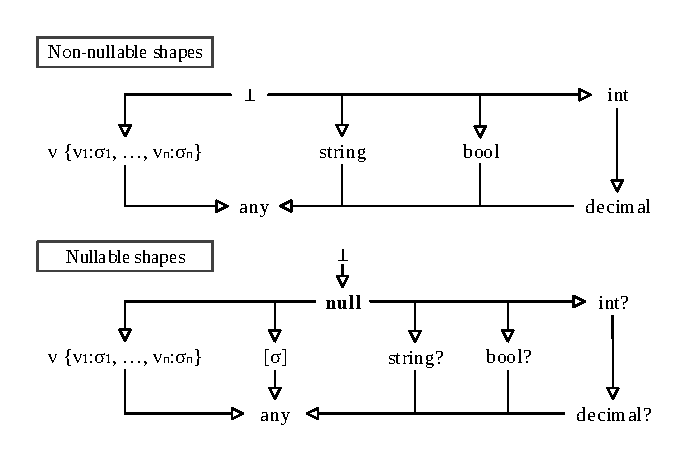
\includegraphics[scale=0.80,trim=5mm 5mm 5mm 5mm,clip]{images/hierarchy.pdf} % left bottom right top
\end{center}
\vspace{-0.5em}
\caption{Subtype relation between structural types}
\label{fig:subtyping-diagram}
\vspace{-0.5em}
\end{figure}

% -------------------------------------------------------------------------------------------------

\subsection{Subtyping relation}
\label{sec:inference-subtyping}

Figure~\ref{fig:subtyping-diagram} provides a basic intuition about the subtyping between
structural types. The upper part shows non-nullable types (with records and primitive types) and 
the lower part shows nullable types with \kvd{null}, collections and optional values. We 
abbreviate $\kvd{option}\langl\sigma\rangl$ as $\sigma?$ and we omit links between the two parts;
any type $\hat{\sigma}$ is a subtype of $\kvd{option}\langl\hat{\sigma}\rangl$.

\begin{definition}
We write $\sigma_1 :> \sigma_2$ to denote that $\sigma_2$ is a subtype of $\sigma_1$. The 
subtyping relation is defined as a transitive reflexive closure of the following rules:

\noindent
\begin{align}
  \label{eq:sub-prim}\tag{P1}
  \ident{float}\,:>\,\ident{decimal}\,&:>\,\ident{int}&\\[-0.2em]
  \label{eq:sub-null}\tag{P2}
  \sigma &:> \kvd{null}  &(\textnormal{iff}~\sigma \neq \hat{\sigma}) 
\end{align}

\noindent
\begin{align}
  \label{eq:sub-opt}\tag{P3}
  \kvd{option}\langl\hat{\sigma}\rangl &:> \hat{\sigma}  &(\textnormal{for all}~\hat{\sigma})\\[-0.2em]
  \label{eq:sub-opt-cov}\tag{P4}
  \kvd{option}\langl\hat{\sigma_1}\rangl &:> 
    \kvd{option}\langl\hat{\sigma_2}\rangl  &(\textnormal{if}~\hat{\sigma_1} :> \hat{\sigma_2}) \\[-0.2em]
  \label{eq:sub-col}\tag{P5}
  [\sigma_1] &:> [\sigma_2]  &(\textnormal{if}~\sigma_1 :> \sigma_2) \\[-0.2em]
  \label{eq:sub-bot}\tag{P6}
  \sigma &:> \bot  &(\textnormal{for all}~\sigma)\\[-0.2em]
  \label{eq:sub-var-top}\tag{P7}
  \kvd{any}\langl \sigma_1, \ldots, \sigma_n\rangl &:> \sigma 
\end{align}

\noindent
\begin{align}
\label{eq:sub-record1}\tag{R1}
\begin{array}{l}
 \nu_?~\{ \nu_1\!:\!\sigma_1, .., \nu_n\!:\!\sigma_n \} :> \\
 \nu_?~\{ \nu_1\!:\!\sigma_1', .., \nu_n\!:\!\sigma_n' \}
\end{array} \qquad ~~~~(\textnormal{if}~\sigma_i :> \sigma_i')
\end{align}
\vspace{-0.8em}
\begin{align}
\label{eq:sub-record2}\tag{R2}
\begin{array}{l}
 \nu_?~\{ \nu_1\!:\!\sigma_1, .., \nu_n\!:\!\sigma_n \} :> \\
 \nu_?~\{ \nu_1\!:\!\sigma_1, .., .., \nu_m\!:\!\sigma_m \}
\end{array} \qquad (\textnormal{when}~m \geq n)
\end{align}
\vspace{-0.8em}
\begin{align}
\label{eq:sub-record3}\tag{R3}
\begin{array}{l}
 \nu_?~\{ \nu_1\!:\!\sigma_1, .., \nu_n\!:\!\sigma_n \} :> \\
 \nu_?~\{ \nu_{\pi(1)}\!:\!\sigma_{\pi(1)}, .., \nu_{\pi(m)}\!:\!\sigma_{\pi(m)} \}
\end{array} ~~(\pi~\textnormal{perm.})
\end{align}
\vspace{-0.8em}
\begin{align}
\label{eq:sub-record4}\tag{R4}
\begin{array}{l}
 \nu_?~\{ \nu_1\!:\!\sigma_1, .., \nu_n\!:\!\sigma_n, \nu_{n+1}\!:\!\kvd{null} \} :> \\
 \nu_?~\{ \nu_1\!:\!\sigma_1, .., \nu_n\!:\!\sigma_n \}
\end{array}
\end{align}
\end{definition}

% --------------------------------------------------------------------------------------------------

\begin{figure*}[t]
\noindent
\begin{equation*}
\boxed{
\begin{array}{c}
\begin{array}{rclcl}
 \tytag &\narrow{=}& \ident{bool} \\
        &\narrow{\lsep}& \ident{string} &\narrow{\lsep}& \ident{number}  \\
        &\narrow{\lsep}& \ident{any}  &\narrow{\lsep}& \ident{collection} \\
        &\narrow{\lsep}& \ident{record} &\narrow{\lsep}& \ident{named}\;~\nu 
\end{array}
%
\quad\;\;\;
%
\begin{array}{rcl}
 \tytagof(\ident{string}) &\narrow{=}& \ident{string}\\
 \tytagof(\ident{bool}) &\narrow{=}& \ident{bool}\\
 \tytagof([\sigma]) &\narrow{=}& \ident{collection}\\
 \tytagof(\hat{\sigma}~\kvd{option}) &\narrow{=}& \tytagof(\hat{\sigma})
\end{array}
%
\;\;
%
\begin{array}{rcl}
 \tytagof(\kvd{any}\langl\sigma_1, \ldots, \sigma_n\rangl) &\narrow{=}& \ident{any}\\
 \tytagof(\{ \nu_1 : \sigma_1, \; \ldots \; , \nu_n : \sigma_n \}) &\narrow{=}& \ident{rec-anon}\\
 \tytagof(\nu\; \{ \nu_1 : \sigma_1, \; \ldots \; , \nu_n : \sigma_n \}) &\narrow{=}& \ident{rec-named}~\nu \\
 \multicolumn{3}{c}{ \tytagof(\sigma) = \ident{number}\quad \sigma \in\{ \ident{int},\ident{decimal},\ident{float} \}  } 
\end{array}
%
\\[3em]
%
\begin{array}{rcll}
 \addopt{\hat{\sigma}} &\narrow{=}& \hat{\sigma}~\kvd{option} &(\textnormal{non-nullable types})\\
 \addopt{\sigma} &\narrow{=}& \sigma &(\textnormal{otherwise})
\end{array}
\qquad\qquad
\begin{array}{rcll}
 \dropopt{\hat{\sigma}~\kvd{option}} &\narrow{=}& \hat{\sigma} &(\textnormal{option})\\
 \dropopt{\sigma} &\narrow{=}& \sigma &(\textnormal{otherwise})
\end{array}
\end{array}
}
\end{equation*}

\begin{equation*}
\hspace{3em}
\inference[(record-1)\;]
  { (\nu_i = \nu'_j) \Leftrightarrow (i = j) \wedge (i \leq k)
      \qquad \forall i\in\{ 1 .. k \}.(\sigma_i \tsep \sigma'_i \vdash \sigma''_i) }
  { \begin{array}{l}
    \nu_? \; \{ \nu_1 \!:\! \sigma_1,  \; \ldots \;, \nu_k \!:\! \sigma_k, \; \ldots \;, \nu_n \!:\! \tau_n \} \tsep
    \nu_? \; \{ \nu'_1 \!:\! \sigma'_1, \; \ldots \;, \nu'_k \!:\! \sigma'_k, \; \ldots \;, \nu'_m \!:\! \tau'_m \} \vdash\\
    \nu_? \; \{ \nu_1 \!:\! \sigma''_1, \; \ldots \; , \nu_k \!:\! \sigma''_k, 
                            \nu_{k+1} \!:\! \addopt{\sigma_{k+1}}, \ldots, \nu_n \!:\! \addopt{\sigma_n},
                            \nu'_{k+1} \!:\! \addopt{\sigma'_{k+1}}, \ldots, \nu'_m \!:\! \addopt{\sigma'_m} \}
    \end{array} }
\end{equation*}
\vspace{-2em}

% union with something else
\begin{equation*}
\textnormal{\footnotesize{(var-1)}}\;\;
\inference
  {\exists i . \tytagof(\sigma_i) = \tytagof(\sigma) & \sigma \tsep \sigma_i \vdash \sigma_i' & \tytagof(\sigma)\neq\ident{any}}
  {\sigma \tsep \kvd{any}\langl\sigma_1, \ldots, \sigma_n\rangl \vdash 
    \kvd{any}\langl\sigma_1, \ldots, \dropopt{\sigma_i'}, \ldots, \sigma_n\rangl}
\;\;
\inference
  {\nexists i . \tytagof(\sigma_i) = \tytagof(\sigma) & \tytagof(\sigma)\neq\ident{any}}
  {\sigma \tsep \kvd{any}\langl\sigma_1, \ldots, \sigma_n\rangl \vdash 
    \kvd{any}\langl\sigma_1, \ldots, \sigma_n, \dropopt{\sigma}\rangl}
\end{equation*}
\vspace{-2em}

% two union types
\begin{equation*}
\begin{array}{l}
\inference[(var-2)\;]
  { (\forall i\in \{ 1 .. k \})\quad \tytagof(\sigma_i) = \tytagof(\sigma'_i) \quad 
    \sigma_i \tsep \sigma_i' \vdash \sigma''_i}
  { \begin{array}{l}
    \kvd{any}\langl \sigma_1, \ldots, \sigma_k,  \ldots, \sigma_n\rangl \tsep 
    \kvd{any}\langl \sigma'_1, \ldots, \sigma'_k, \ldots, \sigma'_m\rangl \vdash\\
    \kvd{any}\langl \sigma''_1, \ldots, \sigma''_k, \sigma_{k+1}, \ldots, \sigma_{n}, \sigma'_{k+1}, \ldots, \sigma'_{m}\rangl
    \end{array} }
\end{array}    
\begin{array}{l}
\inference[(var-3)\;]
  {(\forall i\in\{1,2\}) & \tytagof(\sigma_1) \neq \tytagof(\sigma_2) \\ 
   \tytagof(\sigma_i) \neq \ident{any} & \nexists\sigma_i' . (\sigma_i = \kvd{option}\langl\sigma_i'\rangl)  }
  {\sigma_1 \tsep \sigma_2 \vdash \kvd{any}\langle\dropopt{\sigma_1}, \dropopt{\sigma_2}\rangle}
\end{array}  
\end{equation*}
\vspace{-2em}

\begin{equation*}
\inference[(order-1)\;]
  { \nu_? \; \{ \nu_1 : \sigma_1, \ldots, \nu_n : \sigma_n \} \tsep \sigma \vdash \sigma' }
  { \nu_? \; \{ \nu_{\pi(1)} : \sigma_{\pi(1)}, \ldots, \nu_{\pi(n)} : \sigma_{\pi(n)} \} \tsep \sigma \vdash \sigma' }
\quad
\inference[(order-2)\;]
  { \kvd{any}\langl\sigma_1, \ldots, \sigma_n\rangl \tsep \sigma \vdash \sigma' }
  { \kvd{any}\langl\sigma_{\pi(1)}, \ldots, \sigma_{\pi(n)}\rangl \tsep \sigma \vdash \sigma' }
\quad (\pi~\textnormal{perm.})  
\end{equation*}
\vspace{-2em}

\begin{equation*}
\hspace{3em}
% option types
\inference[(opt)\;]
  {\hat{\sigma_1} \tsep \sigma_2 \vdash \sigma}
  {\kvd{option}\langl\hat{\sigma_1}\rangl \tsep \sigma_2 \vdash \kvd{option}\langl\dropopt{\sigma}\rangl}
\qquad
% primitive types
\inference[(prim)\;]
  {\sigma_1 :> \sigma_2 &
   \tytagof(\sigma_1) = \tytagof(\sigma_2) = \ident{number} }
  {\sigma_1 \tsep \sigma_2 \vdash \sigma_1}\quad
\end{equation*}
\vspace{-2em}

% all rules are symmetric and reflexive
\begin{equation*}
\inference[(list)\;]
  {\sigma_1 \tsep \sigma_2 \vdash \sigma}
  {[\sigma_1] \tsep [\sigma_2] \vdash [\sigma]}
\quad
\inference[(sym)\;]
  {\sigma_1 \tsep \sigma_2 \vdash \sigma}
  {\sigma_2 \tsep \sigma_1 \vdash \sigma}
%
\quad
\begin{array}{l}
 \textnormal{\footnotesize{(refl)}}\;\; \sigma \tsep \sigma \vdash \sigma\\[0.6em]
 % bottom type
 \textnormal{\footnotesize{(bot)}}\;\; \bot \tsep \sigma \vdash \sigma
\end{array}
%
\quad
% null and nullable
 \begin{array}{l}
 \textnormal{\footnotesize{(null-1)}}\;\; \sigma \tsep \kvd{null} \vdash \sigma \quad(\sigma :> \kvd{null}) \\[0.6em]
 \textnormal{\footnotesize{(null-2)}}\;\; \sigma \tsep \kvd{null} \vdash \sigma~\kvd{option} \quad(\sigma :\ngtr \kvd{null})
 \end{array}
\end{equation*}

\caption{Inference judgements that define the common supertype relation}
\label{fig:subtyping-cst}
\end{figure*}

% --------------------------------------------------------------------------------------------------

\noindent
Here is a summary of the key aspects of the definition:
\begin{itemize}
\item Numeric types (\ref{eq:sub-prim}) are ordered by the range they represent;
  \ident{int} is a 32-bit integer, \ident{decimal} has a range of $-1^{29}$ to $1^{29}$ and 
  \ident{float} is a floating-point number (but imprecise).

\item The \kvd{null} type is a subtype of all nullable types (\ref{eq:sub-null}), i.e. all 
  types excluding non-nullable types $\hat{\sigma}$. Any non-nullable type is a 
  subtype of its optional version (\ref{eq:sub-opt}) and both options and collections are 
  covariant (\ref{eq:sub-opt-cov}, \ref{eq:sub-col}).

\item There is a bottom type (\ref{eq:sub-bot}) and variants behave as top types, because
  any type $\sigma$ is a subtype of any variant (\ref{eq:sub-var-top}). There is a range of
  variants (no \emph{single} top type), but any variant is a subtype of variants with fewer tags.

\item As usual, the subtyping on records is covariant (\ref{eq:sub-record1}), subtype can have 
  additional fields (\ref{eq:sub-record2}) and fields can  be reordered (\ref{eq:sub-record3}). 
  Rule (\ref{eq:sub-record4}) is discussed below.
\end{itemize}

\noindent
If we were simply type-checking programs, using variant-annotated top types  
would not add value over having a single top type. However, as shown earlier (\S\ref{sec:providers-xml}), 
the types forming a variant provide a valuable information about the sample document.

A particularly important rule is (\ref{eq:sub-record4}), which, 
together with covariance, states that a supertype can include additional fields, 
provided that their types are nullable (which includes option types). Values of the subtype
will report the null value for these additional fields.
This gives many possible supertypes for a record type: including types with fewer fields and more nullable fields.
This flexiblity will allow us to prefer records-with-extra-nullable-fields
over variants when computing common supertypes. For example, given 
$\{ \ident{name}\!:\!\ident{string} \}$ and $\{ \ident{name}\!:\!\ident{string}, \ident{age}\!:\!\ident{int} \}$,
we find a common supertype $\{ \ident{name}\!:\!\ident{string}, \ident{age}\!:\!\ident{int}~\kvd{option} \}$.
This is a least upper bound (clarified below) and preferred over other common supertypes 
$\kvd{var}\langl \{ \ident{name}\!:\!\ident{string} \}, \{ \ident{name}\!:\!\ident{string}, \ident{age}\!:\!\ident{int} \}\rangl$.

Some of the aspects of our system such as the relationship between numeric types is
based on common industry practice and are to some extent tunable. For example, 
options can be added to always assume that all fields are always nullable.  The default
options may differ according to common practice in different programming communities.

% -------------------------------------------------------------------------------------------------

\begin{figure*}
\noindent
\begin{equation*}
\begin{array}{l}
\ident{asFloat}(i) \,\reduce f\quad(f = i)\\
\ident{asFloat}(d) \reduce f\quad(f = d)\\
\ident{asFloat}(f) \reduce f
\\[0.5em]
\ident{asDec}(i) \,\reduce d\quad(d = i)\\
\ident{asDec}(d) \reduce d
\end{array}
\qquad
\begin{array}{l}
\ident{hasType}(\nu_? \{ \nu_1 \!:\! \sigma_1, \ldots, \nu_n \!:\! \sigma_n \}, \nu'_? \{ \nu'_1\mapsto s_1, \ldots, \nu'_m\mapsto s_m \}) \reduce (\nu_? = \nu'_?) ~\wedge \\
  \quad (~ ((\nu_1 = \nu'_1) \wedge \ident{hasType}(\sigma_1, s_1)) \vee\ldots\vee ((\nu_1 = \nu'_m) \wedge \ident{hasType}(\sigma_1, s_m)) \vee \ldots \vee\\
  \quad ~\; ((\nu_n = \nu'_1) \wedge \ident{hasType}(\sigma_n, s_1)) \vee\ldots\vee ((\nu_n = \nu'_m) \wedge \ident{hasType}(\sigma_n, s_m))~)
\\[0.5em]
\ident{hasType}([\sigma], [s_1; \ldots; s_n]) \reduce \ident{hasType}(\sigma, s_1)\wedge\ldots\wedge\ident{hasType}(\sigma, s_n) \\
\ident{hasType}([\sigma], \kvd{null}) \reduce \kvd{true} \\  
\end{array}  
\end{equation*}
%
\vspace{-0.5em}
%
\begin{equation*}
\begin{array}{l}
\ident{isNull}(\kvd{null}) \reduce \kvd{true} \\
\ident{isNull}(\_) \reduce \kvd{false} 
\\[0.5em]
\ident{getField}(\nu,\nu_i, \nu~\{\ldots, \nu_i=s_i, \ldots\}) \reduce s_i\\
\ident{getField}(\bullet, \nu_i, \{\ldots, \nu_i=s_i, \ldots\}) \reduce s_i\\
\ident{getField}(\nu,\nu', \nu~\{\ldots, \nu_i=s_i, \ldots\}) \reduce \kvd{null}\quad(\nexists i.\nu_i=\nu' )\\
\ident{getField}(\bullet, \nu', \{\ldots, \nu_i=s_i, \ldots\}) \reduce \kvd{null}\quad(\nexists i.\nu_i=\nu' )
\\[0.5em]
\ident{getChildren}([s_1; \ldots; s_n]) \reduce [s_1; \ldots; s_n]  \\  
\ident{getChildren}(\kvd{null}) \reduce [~] 
\end{array}
~
\begin{array}{l}
\ident{hasType}(\ident{string}, t) \reduce \kvd{true} \\
\ident{hasType}(\ident{bool}, s) \reduce \kvd{true} \quad(\textnormal{when}~s\in{\kvd{true},\kvd{false}} )\\
\ident{hasType}(\ident{float}, s) \reduce \kvd{true} \quad(\textnormal{when}~s=i, s=d ~\textnormal{or}~ s=f) \\
\ident{hasType}(\ident{decimal}, s) \reduce \kvd{true} \quad(\textnormal{when}~s=i ~\textnormal{or}~ s=f) \\
\ident{hasType}(\ident{int}, i) \reduce \kvd{true}\\
\ident{hasType}(\kvd{option}\langl\sigma\rangl, s) \reduce \ident{hasType}(\sigma,s) \\
\ident{hasType}(\kvd{option}\langl\sigma\rangl, s) \reduce \kvd{true} \\
\ident{hasType}(\kvd{any}\langl\ldots\rangl, s) \reduce \kvd{true} \\
\ident{hasType}(\_, \_) \reduce \kvd{false} \\
\end{array}
\end{equation*}

\caption{Reduction rules for conversion functions}
\label{fig:op-conversions}
\end{figure*}

% -------------------------------------------------------------------------------------------------

\subsection{Common supertype relation}
\label{sec:inference-commonsuper}

Given two structural types, the \emph{common supertype} relation finds a least upper bound
(Theorem~\ref{thm:lub}). When possible, it avoids variant types and prefers records 
(Corollary~\ref{thm:no-unions}), which is important for usability as discussed earlier
(\S\ref{sec:providers-json}). 

\begin{definition}
A \emph{common supertype} of types $\sigma_1$ and $\sigma_2$ is a type $\sigma$, written 
$\sigma_1 \triangledown \sigma_2 \vdash \sigma$, obtained according to the inference rules in 
Figure~\ref{fig:subtyping-cst}.
\end{definition}

\noindent
When finding a common supertype of records (\emph{record-1}), we return a record that has the 
union of their fields. The types of shared fields become common supertypes of their respective 
types while fields that are present in only one record are marked as optional. The (\emph{order-1})
rule lets us reorder fields.

Although all variants are mutual subtypes, we find one that best represents the sample. We avoid
nested variants and limit the number of cases. This is done by grouping types 
that have a common supertype which is not a variant. For example, rather than inferring 
$\kvd{any}\langl\ident{int}, \kvd{any}\langl\ident{bool}, \ident{decimal}\rangl\rangl$, 
our algorithm finds the common supertype of $\ident{int}$ and $\ident{decimal}$ and produces 
$\kvd{any}\langl\ident{decimal},\ident{bool}\rangl$. To identify types that have a common supertype 
which is not a variant, we group the types by a tag. The tag of a type is obtained using a function 
\tytagof{(-)}. The function is not defined on $\bot$ and $\kvd{null}$ as those are handled by the 
(\emph{bot}) and (\emph{null-1}) or (\emph{null-2}).

The handling of variants is specified using three rules. When combining a non-variant and a
variant (\emph{var-1}), the variant may or may not already contain a case with the tag of the other
type. If it does, the two types are combined, otherwise a new case is added.
When combining two variants (\emph{var-2}), we group the cases that have a shared tags.
Finally, (\emph{var-3}) covers the case when we are combining two distinct non-variant types.
As variants implicitly permit \kvd{null} values, we use an auxiliary function $\dropopt{-}$ to
make nullable types non-nullable (when possible) to simplify the type.

The remaining rules are straightforward. For collections and options, we find the common supertype 
of the contained value(s); for compatible primitive types, we choose their supertype (\emph{prim})
and a common supertype with \kvd{null} is either the type itself (\emph{null-1}) or an option 
(\emph{null-2}).

\paragraph{Properties.}
The partially ordered set of types does not have a \emph{unique} least upper bound, but it does 
have a least upper bound with respect to an equivalence between mutual subtypes. The common 
supertype relation is well-defined (Theorem~\ref{thm:func}) and finds the least upper bound 
(Theorem~\ref{thm:lub}). 

\begin{definition}
Types $\sigma_1$, $\sigma_2$ are \emph{equivalent}, written $\sigma_1 \equiv \sigma_2$ iff
they are mutual subtypes, i.e. $\sigma_1 <: \sigma_2 \wedge \sigma_1 :> \sigma_2$.
An equivalence class of a type $\sigma$ is $\mathcal{E}(\sigma) = \{ \sigma' \;|\; \sigma\equiv\sigma' \}$.
\end{definition}

\noindent
The equivalence class $\mathcal{E}$ sheds light on the structure of structural types. It defines
a lattice with bottom $\{ \bot \}$ and top (set of all variant types). It also joins records with
reordered fields (of same names and types) and types that contain other equivalent types (e.g.~a
lists containing variant values).

\begin{theorem}[Function]
\label{thm:func}
\raggedright
For all $\sigma_1$ and $\sigma_2$ there exists exactly one $\sigma$ such that 
$\sigma_1 \triangledown \sigma_2 \vdash \sigma$.
Furthermore, if $\sigma_1 \triangledown \sigma_2 \vdash \sigma'$
then it holds that $\sigma :> \sigma'$ and $\sigma' :> \sigma$.
\end{theorem}
\begin{proof}
The pre-conditions of rules in Figure~\ref{fig:subtyping-cst} are disjoint, with the exception 
of (\emph{order}), (\emph{sym}) and (\emph{refl}). These rules produce types that are subtypes
of each other and this property is preserved by rules that use $\triangledown$ recursively.
\end{proof}

\begin{theorem}[Least upper bound]
\label{thm:lub}
\raggedright
If $\sigma_1 \triangledown \sigma_2 \vdash \sigma$ then $\sigma$ is a least upper bound, i.e. 
$\sigma :> \sigma_1$ and $\sigma :> \sigma_2$ and for all $\sigma'$ such that $\sigma' :> \sigma_1$
and $\sigma' :> \sigma_2$, it holds that $\sigma' :> \sigma$.
\end{theorem}
\begin{proof}
By induction over $\vdash$. Note that the algorithm never produces nested variant or nested
option. When one type is variant, the only common supertype is also a variant (\emph{var-2}); 
for (\emph{var-3}) no other common supertype exists because the two types have distinct 
tags and are not options.
\end{proof}

\begin{corollary}
\label{thm:no-unions}
Given $\sigma_1, \sigma_2, \sigma$ such that $\sigma :> \sigma_1$ and $\sigma :> \sigma_2$ and 
$\sigma$ is not a variant, then $\sigma_1 \tsep \sigma_2 \vdash \sigma'$ 
and $\sigma' \equiv \sigma$.
\end{corollary}
\begin{proof}
Consequence of Theorem~\ref{thm:lub} and the fact that the set of all variants is the
top element of $\mathcal{E}$.
\end{proof}



% ==================================================================================================
% 
%    #######
%    #        ####  #####  #    #   ##   #      # ######   ##   ##### #  ####  #    #
%    #       #    # #    # ##  ##  #  #  #      #     #   #  #    #   # #    # ##   #
%    #####   #    # #    # # ## # #    # #      #    #   #    #   #   # #    # # #  #
%    #       #    # #####  #    # ###### #      #   #    ######   #   # #    # #  # #
%    #       #    # #   #  #    # #    # #      #  #     #    #   #   # #    # #   ##
%    #        ####  #    # #    # #    # ###### # ###### #    #   #   #  ####  #    #
%
% ==================================================================================================

\section{Formalising type providers}
\label{sec:formal}

In this section, we build the theoretical framework for proving relativised type safety of 
structural type providers. We discuss the runtime representation of documents and 
primitive operations (\S\ref{sec:formal-convert}), we embed these into a formal model of an F\# 
subset (\S\ref{sec:formal-ff}) and we describe how structural type providers turn
inferred structural types into F\# types (\S\ref{sec:formal-tp}).

% -------------------------------------------------------------------------------------------------

\subsection{Structural values and conversions}
\label{sec:formal-convert}

We represent JSON, XML and CSV documents using the same \emph{structural value}. Structural 
values are first-order and can be one of the following cases:
%
\begin{equation*}
\begin{array}{lcl}
 s &\narrow{=}& i \lsep d \lsep f \lsep t \lsep \kvd{true} \lsep \kvd{false} \lsep \kvd{null} \\[0.1em]
   &\narrow{|}& [s_1; \ldots; s_n] \lsep \nu_?\{ \nu_1 \mapsto s_1, \ldots, \nu_n \mapsto s_n \}
\end{array}
\end{equation*}
%
The first few cases represent primitive values ($i$ for integers, $d$ for decimals, $f$ for floating
point numbers and $t$ for strings) and the \kvd{null} value. A collection is written as a 
list of values in square brackets. A record starts with an optional name $\nu_?$, followed by a 
sequence of field assignments $\nu_i \mapsto s_i$.

As indicated by the subtyping, our system permits certain runtime conversions (e.g.~an integer
\num{1} can be treated as a floating-point \num{1.0}). The following primitive operations 
implement the conversions and other helpers:
%
\begin{equation*}
\begin{array}{lcl}
 op  &\narrow{=}& \ident{asDec}(s) \lsep \ident{asFloat}(s) \lsep \ident{getChildren}(s) \\
     &\narrow{|}& \ident{getField}(\nu?, \nu, s) \lsep \ident{isNull}(s) \lsep \ident{hasType}(\sigma, s)
\end{array}
\end{equation*}
%
The operations are used in code generated by type providers. Their behavior is defined
by the rules in Figure~\ref{fig:op-conversions}. The conversion functions (\ident{asDec}
and \ident{asFloat}) only perform conversions required by the subtyping relation (our actual 
implementation is more lax and performs additional conversions).

The \ident{getField} operation is used to access a field of a record. The operation ensures that
the actual record name matches the expected name (we write $\bullet$ for the name of an unnamed 
record). The \ident{getChildren} operation returns elements of a list and turns \kvd{null} into 
an empty collction.

Finally, we also define two helper functions. The \ident{isNull} operation is used to check whether 
value is \kvd{null} and \ident{hasType} is a runtime type test. The most complex case is handling 
of records where we check that for each field $\nu_1, \ldots, \nu_n$ in the type, the actual record 
value has a field of the same name with a matching type. The last line defines a ``catch all'' 
pattern, which returns \kvd{false} for all remaining cases. Although not elenegantly, the rules 
can be expressed using just Featherweight F\#, discussed in the next section.

% -------------------------------------------------------------------------------------------------

\begin{figure}
\noindent
\begin{equation*}
\begin{array}{rl}
 \textnormal{\footnotesize{(member)}}&
 \hspace{-0.4em}
 \inference
 { \kvd{type}~C(\overline{x:\tau})=\ldots \kvd{member}~N_i : \tau_i = e_i \ldots }
 { (\kvd{new}~C(\overline{v})).N_i \reduce e_i[\overline{x} \leftarrow \overline{v}] }\\
 \\
 \textnormal{\footnotesize{(eq1)}}&
 v=v\reduce\kvd{true} \qquad \textnormal{\footnotesize{(eq2)}}~~v=v'\reduce\kvd{false}\\
 \\
 \textnormal{\footnotesize{(cond1)}}&
 \hspace{-0.4em}
 \kvd{if}~\kvd{true}~\kvd{then}~e_1~\kvd{else}~e_2 ~\reduce~ e_1 \\
 \\
 \textnormal{\footnotesize{(cond2)}}&
 \hspace{-0.4em}
 \kvd{if}~\kvd{false}~\kvd{then}~e_1~\kvd{else}~e_2 ~\reduce~ e_2 \\
 \\
 \textnormal{\footnotesize{(match1)}}&
 \hspace{-1em}
 \begin{array}{l}
  \kvd{match}~\ident{None}~\kvd{with} \\
  \ident{Some}(x) \rightarrow e_1 \,|\, \ident{None} \rightarrow e_2
 \end{array} \hspace{-0.5em} ~\reduce~ e_2 \\
 \\
 \textnormal{\footnotesize{(match2)}}&
 \hspace{-1em}
 \begin{array}{l}
    \kvd{match}~\ident{Some}(v)~\kvd{with} \\
    \ident{Some}(x) \rightarrow e_1 \,|\, \ident{None} \rightarrow e_2
 \end{array} \hspace{-0.5em} ~\reduce~ e_1[x\leftarrow v]\\
 \\
 \textnormal{\footnotesize{(match3)}}&
 \hspace{-1em}
 \begin{array}{l}
  \kvd{match}~[v_1;\ldots;v_n]~\kvd{with} \\[0em]
  [x_1;\ldots;x_m ] \rightarrow e_1 \,|\, \_ \rightarrow e_2
 \end{array} \hspace{-0.5em} ~\reduce~ e_2\quad(m\neq n) \\
 \\
 \textnormal{\footnotesize{(match4)}}&
 \hspace{-1em}
 \begin{array}{l}
  \kvd{match}~[v_1;\ldots;v_n]~\kvd{with} \\[0em]
  [x_1;\ldots;x_n ] \rightarrow e_1 \,|\, \_ \rightarrow e_2
 \end{array} \hspace{-0.5em} ~\reduce~ e_1[\overline{x}\leftarrow\overline{v}] \\
 \\
 \textnormal{\footnotesize{(map)}}&
 \hspace{-0.4em}
 \ident{map}~(\lambda x.e)~[v_1; \ldots] ~\reduce~ [e[x\leftarrow v_1]; \ldots] \\
 \\
 \textnormal{\footnotesize{(ctx)}}&
 \hspace{-0.4em}
  E[e] \reduce E[e'] \qquad\qquad(\textnormal{when}~e \reduce e')\\
\end{array}
\end{equation*}

\caption{Featherweight F\# -- Remaining reduction rules}
\label{fig:ff-reduction}
\vspace{-1em}
\end{figure}

% -------------------------------------------------------------------------------------------------

\subsection{Featherweight F\#}
\label{sec:formal-ff}

We now extend the semantics discussed so far and add a minimal subset of F\# needed to model F\# 
Data. Type providers use classes and so we focus on the F\# object model and combine aspects of SML 
\cite{sml} and Featherweight Java \cite{fwjava}. 

We only need classes with parameter-less members and without inheritance. A class has a single 
implicit constructor and the declaration closes over constructor parameters. To avoid including all 
of ML, we only pick constructs for working with options and lists that we need later.
%
\begin{equation*}
\begin{array}{rcl}
 \tau &\narrow{=}& \ident{int} \lsep \ident{decimal} \lsep \ident{float} \lsep \ident{bool} \lsep \ident{string} \\[0.0em]
      &\narrow{|}& C \lsep \ident{StructVal} \lsep \ident{list}\langl\tau\rangl \lsep \ident{option}\langl\tau\rangl \\[0.6em]
 L &\narrow{=}& \kvd{type}~C(\overline{x:\tau}) = \overline{M} \\[0.0em]
 M &\narrow{=}& \kvd{member}~N:\tau=e
\end{array}
\end{equation*}

\noindent
\begin{equation*}
\begin{array}{rcl}
 v &\narrow{=}& s \lsep \ident{None} \lsep \ident{Some}(v) \lsep \kvd{new}~C(\overline{v}) \lsep [v_1; \ldots; v_n] \\[0.0em]
 e &\narrow{=}& s \lsep op \lsep e.N \lsep \kvd{new}~C(\overline{e}) \lsep {\kvd{if}~e_1~\kvd{then}~e_2~\kvd{else}~e_3}\\
   &\narrow{|}& \ident{None} \lsep\kvd{match}~e~\kvd{with}~\ident{Some}(x) \rightarrow e_1 \,|\, \ident{None} \rightarrow e_2 \\
   &\narrow{|}& \ident{Some}(e) \lsep [e_1;\ldots;e_n]\lsep \ident{map}~(\lambda x\rightarrow e_1)~e_2\\
   &\narrow{|}& e = e \lsep \kvd{match}~e~\kvd{with}~[x_1; \ldots; x_n] \rightarrow e_1 \,|\, \_ \rightarrow e_2
\end{array}
\end{equation*}

\noindent
The type \ident{StructVal} is a type of all structural values $s$. A class
definition $L$ consists of a constructor and zero or more members. Values $v$ include 
previously defined structural values $s$ and values for the option and list type; finally 
expressions $e$ include previously defined operations $op$, class construction, member access, 
conditionals and expressions for working with option values and lists. We include 
\ident{map} as a special construct to avoid making the language too complex.

Next, we define the reduction relation and (a fragment of) type checking for Featherweight F\#.
The language presented here is intentionally incomplete. We only define parts needed to prove
the relativized safety property (\S\ref{sec:safety}).

\paragraph{Reduction.}
The reduction relation is of the form $e \reduce e'$. We also write 
$e \reduce^{*} e'$ to denote the reflexive and transitive closure of $\reduce$. The reduction rules
for operations $op$ were discussed earlier. Figure~\ref{fig:ff-reduction} shows the remaining
rules.

The (\emph{ctx}) rule performs a reduction inside a sub-expression specified by an evaluation context.
This models the eager evaluation of F\#. An evaluation context $E$ is defined as:

\vspace{0.5em}
\noindent
\begin{equation*}
\begin{array}{l}
\hspace{-0.5em}
\begin{array}{rcl}
 E &\narrow{=}& [\overline{v};E;\overline{e}] \lsep E.N \lsep \kvd{new}~C(\overline{v}, E, \overline{e})\\[0.1em]
   &\narrow{|}& \ident{map}~(\lambda x\rightarrow e)~E \lsep \kvd{if}~E~\kvd{then}~e_1~\kvd{else}~e_2 \\[0.1em]
   &\narrow{|}& \ident{Some}(E) \lsep f(E) \lsep E = e \lsep v = E \\[0.1em]
   &\narrow{|}& \kvd{match}~E~\kvd{with}~\ident{Some}(x) \rightarrow e_1 \,|\, \ident{None} \rightarrow e_2 \\[0.1em]
   &\narrow{|}& \kvd{match}~E~\kvd{with}~[x_1; \ldots; x_n] \rightarrow e_1 \,|\, \_ \rightarrow e_2
\end{array} \\[3em]
f \in \{ \ident{asDec}, \ident{asFloat}, \ident{getField}, \ident{getChildren}, \ident{isNull}, \ident{hasType} \}
\end{array}
\end{equation*}

\noindent
The evaluation first reduces arguments of functions and the evaluation proceeds from left to right 
as denoted by $\overline{v}, E, \overline{e}$ in constructor arguments or $\overline{v};E;\overline{e}$
in list initialization.

We write $e[\overline{x} \leftarrow \overline{v}]$ for the result of replacing variables $\overline{x}$ by
values $\overline{v}$ in an expression. The (\emph{member}) rule reduces a member access using a class 
definition in the assumption to obtain the body of a member. The remaining six rules
give standard reductions for conditionals and pattern matching.

We omit expressions $e \vee e$ and $e \wedge e$ that are used in Figure~\ref{fig:op-conversions}, 
but those can be easily defined as syntactic sugar using \kvd{if}. All expressions reduce to a value in a 
finite number of steps or get stuck due to an error condition. An error condition can be a wrong 
argument passed to conditional, pattern matching or one of the primitives from Figure~\ref{fig:op-conversions}.

% -------------------------------------------------------------------------------------------------

\begin{figure}
\noindent  
\begin{equation*}
\inference
  {L; \Gamma \vdash e_1 : \ident{StructVal}}
  {L; \Gamma \vdash [e_1; \ldots; e_n]:\ident{StructVal}}
\quad  
\inference
  {~}
  {L; \Gamma \vdash n : \ident{int}}
\end{equation*}
\begin{equation*}
\inference
  {L; \Gamma \vdash e_1 : \tau}
  {L; \Gamma \vdash [e_1; \ldots; e_n]:\ident{list}\langl\tau\rangl}
\quad
\inference
  {~}
  {L; \Gamma \vdash s : \ident{StructVal}}
\end{equation*}
\vspace{0.5em}
\begin{equation*}
\inference
  {L; \Gamma \vdash e : C \\ \kvd{type}~C(\overline{x:\tau}) = ..\;\kvd{member}~N_i : \tau_i = e_i\;.. \in L}
  {L; \Gamma \vdash e.N_i:\tau_i}
\end{equation*}
\vspace{0.25em}
\begin{equation*}
\inference
  {L; \Gamma \vdash e_i : \tau_i & \kvd{type}~C(x_1:\tau_1, \ldots, x_n:\tau_n) = \ldots \in L}
  {L; \Gamma \vdash \kvd{new}~C(e_1, \ldots, e_n):C}
\end{equation*}

\caption{Featherweight F\# -- Fragment of type checking}
\label{fig:ff-typecheck}
\end{figure}

% -------------------------------------------------------------------------------------------------

\paragraph{Type checking.} 
Typing rules in Figure~\ref{fig:ff-typecheck} are written using a judgement
$L; \Gamma \vdash e : \tau$ where the context also contains a set of class declarations $L$.
The rules demonstrate the key differences from Standard ML and Featherweight Java:
%
\begin{itemize}
\item[--] All structural values $s$ have the type \ident{StructVal}, but some have other types
  (Booleans, strings, integers, etc.) as illustrated by the rule for $n$.
  For other values, \ident{StructVal} is the only type -- this includes records and \kvd{null}.
\item[--] A list containing other structural values $[s_1; \ldots; s_n]$ has a type \ident{StructVal},
  but can also have the $\ident{list}\langl\tau\rangl$ type. Conversely, lists that contain
  non-structural values like objects or options are not of type \ident{StructVal}.
\item[--] Operations $op$ (omitted) are treated as functions, accepting 
  \ident{StructVal} and producing an appropriate result type.
\item[--] Rules for checking class construction and member access are similar to corresponding
  rules of Featherweight Java.  
\end{itemize}
%
An important part of Featherweight Java that is omitted here is the checking of type declarations
(ensuring the members are well-typed). We consider only classes generated by our type providers 
and those are well-typed by construction.

% -------------------------------------------------------------------------------------------------

\begin{figure*}
\noindent
\begin{equation*}
\quad\qquad\boxed{
\begin{array}{rcl}
 \nameoftag(\ident{string}) &\narrow{=}& \ident{String} \\
 \nameoftag(\ident{bool}) &\narrow{=}& \ident{Boolean} \\
\end{array}
\qquad
\begin{array}{rcl}
 \nameoftag(\ident{number}) &\narrow{=}& \ident{Number} \\
 \nameoftag(\ident{collection}) &\narrow{=}& \ident{List} \\
\end{array}
\qquad
\begin{array}{rcl}
 \nameoftag(\ident{record}) &\narrow{=}& \ident{Record} \\
 \nameoftag(\ident{named}\;\nu) &\narrow{=}& \nu \\
\end{array}
}
\end{equation*}

\begin{multicols}{2}
% Primitive structural types become corresponding F# types and conversion is inserted
\noindent
\begin{equation*}
\begin{array}{l}
 \sem{\sigma_p}_e = \tau_p,op(e),\emptyset\quad\textnormal{where}~\tau_p = \sigma_p \\[0.2em]
\quad\sigma_p, op\in  \{~(\ident{decimal},\ident{asDec}), (\ident{float},\ident{asFloat})~\}
\end{array}
\end{equation*}
%
% Records become classes
\begin{equation*}
\begin{array}{l}
 \sem{\,\nu_? \{ \nu_1 : \sigma_1, \ldots, \nu_n : \sigma_n \}\,}_e = \\[0.1em]
 \quad C, \kvd{new}~C(e), L_1\cup\ldots\cup L_n\cup\{ L \}\quad\textnormal{where}\\[0.6em]
 \qquad \;\;C~\textnormal{is a fresh class name} \\[0.1em]
 \qquad \;\,\,L = \kvd{type}~C(v:\ident{StructVal})~=~M_1\ldots M_n  \\[0.1em]
 \qquad M_i = \kvd{member}~\nu_i:\tau_i=e_i\\[0.1em]
 \qquad \tau_i, e_i, L_i = \sem{\sigma_i}_{e'},\;\; e'=\ident{getField}(\nu_?, \nu_i, e)\\[0.6em]
\end{array}
\end{equation*}
%
% Collections
\begin{equation*}
\begin{array}{l}
 \sem{\,[\sigma]\,}_e = \ident{list}\langl\tau\rangl, e_b, L \;\;\textnormal{where}\\[0.4em]
 \qquad e_b = \ident{map}~(\lambda x\rightarrow e')~(\ident{getChildren}(e)) \\[0.1em]
 \qquad \tau, e', L = \sem{\hat{\sigma}}_x
\end{array}
\end{equation*}
%
% Anything else
\begin{equation*}
\begin{array}{l}
 \sem{\bot}_e = \sem{\kvd{null}}_e = \ident{StructVal}, e, \emptyset
\end{array}
\end{equation*}

\noindent
\begin{equation*}
\hspace{-2.5em}
\begin{array}{l}
 \sem{\sigma_p}_e = \tau_p,e,\emptyset\quad\textnormal{where}~\tau_p = \sigma_p \\[0.2em]
\quad\sigma_p \in  \{~ \ident{string},\ident{bool},\ident{int}~\}\\[0.6em]
\end{array}
\end{equation*}
%
% Sum type
\begin{equation*}
\hspace{-2.5em}
\begin{array}{l}
 \sem{\,\kvd{any}\langl\sigma_1, \ldots, \sigma_n\rangl\,}_e = \\[0.1em]
 \quad C, \kvd{new}~C(e), L_1\cup\ldots\cup L_n\cup\{ L \}\;\;\textnormal{where}\\[0.6em]
 \qquad \;\;C~\textnormal{is a fresh class name} \\[0.1em]
 \qquad \;\,\,L = \kvd{type}~C(v:\ident{StructVal})~=~M_1\ldots M_n \\[0.1em]
 \qquad M_i = \kvd{member}~\nu_i:\ident{option}\langl\tau_i\rangl=\\[0.1em]
 \hspace{5.8em}  \kvd{if}~\ident{hasType}(\sigma_i, v)~\kvd{then}~
     \ident{Some}(e_i)~\kvd{else}~\ident{None} \\[0.1em]
 \qquad \tau_i, e_i, L_i = \sem{\sigma_i}_e,\;\; t_i = \tytagof{(\sigma_i)},\;\; \nu_i=\nameoftag{(t_i)}
\end{array}
\end{equation*}
%
% Option values
\begin{equation*}
\hspace{-2.5em}
\begin{array}{l}
 \sem{\hat{\sigma}\;\,\kvd{option}}_e = \\[0.2em]
 \hspace{1.25em} \ident{option}\langl\tau\rangl, \kvd{if}~\ident{isNull}~e~\kvd{then}~\ident{None}~\kvd{else}~\ident{Some}(e'), L\\[0.2em] 
 \hspace{1.25em} \textnormal{where}~\tau, e', L = \sem{\hat{\sigma}}_e
\end{array}
\end{equation*}
\end{multicols}

\caption{Type provider -- generation of featherweight F\# types from inferred structural types}
\label{fig:tp-generation}
\vspace{-0.5em}
\end{figure*}

% -------------------------------------------------------------------------------------------------

\subsection{Type providers}
\label{sec:formal-tp}

So far, we defined the type inference algorithm which produces a structural type $\sigma$ from one 
or more sample documents (\S\ref{sec:inference}) and we defined a simplified model of evaluation
of F\# (\S\ref{sec:formal-ff}) and F\# Data runtime (\S\ref{sec:formal-tp}). In this section, we 
define how the type providers work, linking the two parts.

All F\# Data type providers take (one or more) sample documents, infer a common supertype $\sigma$
and then use it to generate F\# types that are exposed to the programmer\footnote{The actual 
implementation provides \emph{erased types} as described in \cite{fsharp-typeprov}. Here, we treat 
the code as actually generated. This is an acceptable simplification, because F\# Data type providers 
do not rely on laziness that is available through erased types.}. 

\paragraph{Type provider mapping.}
The type provider produces an F\# type $\tau$ together with an expression that wraps an input
value (of type \ident{StructVal}) as a value of type $\tau$ and a collection of class definitions. 
We express it using the following mapping:
%
\begin{equation*}
\sem{-}_{-} : (\sigma\times e) \rightarrow (\tau \times e' \times L)
\end{equation*}
%
The mapping $\sem{\sigma}_e$ takes an inferred structural type $\sigma$ and an expression $e$, 
which represents code to obtain a structural value that is being wrapped. It returns an F\# type 
$\tau$, an expression $e'$ which constructs a value of type $\tau$ using $e$ and also a set of 
generated class definitions $L$.

Figure~\ref{fig:tp-generation} shows the rules that define $\sem{-}_{-}$. Primitive types are all
handled by two rules -- for \ident{decimal} and \ident{float}, we insert a call to an appropriate 
conversion function from Figure~\ref{fig:op-conversions}.
Handling of records is more interesting. We generate a class $C$ that takes a structural value as constructor
parameter. For each record field, we generate a new member with the same name as the field\footnote{The actual
F\# Data implementation also capitalizes the names.}. The body of the member calls \ident{getField} and then
wraps this expression using $\sem{\sigma_i}$ which maps the field (structural value of type $\sigma_i$) into 
an F\# value of type $\tau_i$. The returned expression creates a new instance of $C$ and the mapping returns 
the class $C$ together with all recursively generated definitions. Note that the class
name $C$ is not directly accessed by the user and so we can use arbitrary name, although the actual 
implementation in F\# Data attempts to infer a reasonable name\footnote{For example, in 
\ident{\{\str{person}:\{\str{name}:\str{Tomas}\}\}}, the nested record will be named \ident{Person}
based on the name of the parent record field.}.

A collection type becomes an F\# $\ident{list}\langl\tau\rangl$. The returned expression calls \ident{getChildren}
(which turns \kvd{null} into an empty list) and then uses \ident{map} to convert nested values to 
values of an F\# type $\tau$. The handling of option type is similar; if the value is not \kvd{null},
we wrap the recursively generated conversion expression $e'$ in the \ident{Some} constructor.

As discussed earlier, variant types are also generated as F\# classes with properties. Given a variant
$\kvd{any}\langl\sigma_1, \ldots, \sigma_n\rangl$, we get corresponding F\# types $\tau_i$ and generate 
$n$ members of type $\ident{option}\langl \tau_i\rangl$. When the member is accessed, we need to perform
a runtime type test using \ident{hasType} to ensure that the value has the right type (similarly to runtime 
type conversions from the top type in languages like Java). If the type matches, a \ident{Some} value is 
returned. The type inference algorithm also guarantees that there is only one case for each type tag 
(\S\ref{sec:inference-commonsuper}) and so we can use the tag when naming the generated member 
(using the \ident{nameof} function).

\paragraph{Example 1.}
To illustrate how the mechanism works, we consider two examples. First, assume 
that the inferred type is a record  
$\{~\ident{Age}\!:\!\kvd{option}\langl\ident{int}\rangl, \ident{Name}\!:\!\ident{string}~ \}$. 
The rules from Figure~\ref{fig:tp-generation} produce the following class:
%
\begin{equation*}
\begin{array}{l}
 \kvd{type}~\ident{Person}(\ident{v}:\ident{StructVal})~= \\[0.1em]
 \quad \kvd{member}~\ident{Age}~:~\ident{option}\langl\ident{int}\rangl~= \\[0.1em]
 \qquad \kvd{if}~\ident{isNull}~(\ident{getField}(\ident{Person},\ident{Age}, \ident{v}))~\kvd{then}~\ident{None} \\[0.1em]
 \qquad \kvd{else}~\ident{Some}(\ident{asInt}(\ident{getField}(\ident{Person},\ident{Age}, \ident{v}))) \\[0.1em]
 \quad \kvd{member}~\ident{Name}~:~\ident{string}~= \\[0.1em]
 \qquad \ident{asStr}(\ident{getField}(\ident{Person},\ident{Name}, \ident{v}))
\end{array}
\end{equation*}
%
The body of the \ident{Age} member is produced by the case for optional types applied to an expression
$\ident{getField}(\ident{Person},\ident{Age},v)$. If the returned field is not \kvd{null}, then the member
calls \ident{asInt} (produced by the case for primitive types) and wraps the result in \ident{Some}.
Note that \ident{getField} is defined even when the field does not exist, but it returns 
\kvd{null}. This lets us treat missing fields as optional. An F\# type corresponding to the (structural)
record is \ident{Person} and given a structural value $s$, we create a \ident{Person} value by calling 
$\kvd{new}~\ident{Person}(s)$.

\paragraph{Example 2.} The second example illustrates the remaining types including collections and 
variants. Reusing \ident{Person} from the previous example, consider 
$[\kvd{any}\langl\ident{Person},\ident{string}\rangl]$, a collection which contains a mix 
of \ident{Person} and string values:
%
\begin{equation*}
\begin{array}{l}
 \kvd{type}~\ident{PersonOrString}(v:\ident{StructVal})~= \\[0.1em]
 \quad \kvd{member}~\ident{Person}~:~\ident{option}\langl\ident{Person}\rangl~= \\[0.1em]
 \qquad \kvd{if}~\ident{hasType}(\{\ident{Age}\!:\!\kvd{option}\langl\ident{int}\rangl, \ident{Name}\!:\!\ident{string}\}, v)~\\[0.1em]
 \qquad\quad \kvd{then}~\ident{Some}(\kvd{new}~\ident{Person}(v))~\kvd{else}~\ident{None} \\[0.1em]
 \quad \kvd{member}~\ident{String}~:~\ident{option}\langl\ident{string}\rangl~= \\[0.1em]
 \qquad \kvd{if}~\ident{hasType}(\ident{string}, v)~\\[0.1em]
 \qquad\quad \kvd{then}~\ident{Some}(\ident{asStr}(v))~\kvd{else}~\ident{None}
\end{array}
\end{equation*}
%
The type provider maps the structural type to an F\# type $\ident{list}\langl\ident{PersonOrString}\rangl$. 
Given a structural document value $s$, the code to obtain the wrapped F\# value is:
%
\begin{equation*}
\ident{map}~(\lambda x\rightarrow\kvd{new}~\ident{PersonOrString}(x))~(\ident{getChildren}(s))
\end{equation*}
%
The \ident{PersonOrString} type contains one member for each of the variant case. In the body, they
check that the value has the correct type using \ident{hasType}. This also implicitly handles \kvd{null}
by returning \kvd{false}. As discussed earlier, variants provide easy access to the known cases
(\ident{string} or \ident{Person}), but they are robust with respect to unexpected inputs.

% --------------------------------------------------------------------------------------------------

\subsection{Inferring types from values}
\label{sec:formal-inferval}

The common supertype algorithm (\S\ref{sec:inference}) is at the core of the type inference 
for structural values, but we have not yet clarified how it is used. Given a JSON, XML or CSV 
document, F\# Data constructs a structural value $s$ from the sample. The following defines a mapping 
$\semalt{s_1,\ldots,s_n}$ which turns a collection of sample values $s_1, \ldots, s_n$ into a 
structural type $\sigma$:

\noindent
\begin{equation*}
\begin{array}{rclcrclcrcl}
 \semalt{i} &\narrow{=}& \ident{int} && \semalt{d} &\narrow{=}& \ident{decimal} && \semalt{b} &\narrow{=}& \ident{bool}\\
 \semalt{f} &\narrow{=}& \ident{float} && \semalt{t} &\narrow{=}& \ident{string} && \semalt{\kvd{null}}  &\narrow{=}& \kvd{null}\\
\end{array}
\end{equation*}
\noindent
\vspace{-0.5em}
\begin{equation*}
\begin{array}{l}
 \semalt{s_1, \ldots, s_n} = \sigma_n \quad\textnormal{where}\\[0.1em]
 \qquad\sigma_0 = \bot,~ \forall i\in \{ 1.. n \}.~ \sigma_{i-1} \triangledown \semalt{s_i} \vdash \sigma_i
 \\[0.5em]
 \semalt{[s_1; \ldots; s_n]} = [\semalt{s_1, \ldots, s_n}]
 \\[0.5em]
 \semalt{\nu?~\{ \nu_1 \mapsto s_1, \ldots, \nu_n \mapsto s_n \}} =\\[0.1em]
 \qquad\nu?~\{ \nu_1:\semalt{s_1}, \ldots, \nu_n :\semalt{s_n} \}
\end{array}
\end{equation*}
%
We overload the notation and write $\semalt{s}$ when inferring type from a single value. Primitive 
values are mapped to their corresponding types. For records, we return a type with field types 
inferred based on individual values. 

When infering a value from multiple samples, we use the common supertype relation to find a common 
type for all values (starting with $\bot$). This operation is used at the top-level (when calling 
a type provider with multiple samples) and also when inferring the type of a collection.



% ==================================================================================================
%
%    #######
%       #    #   # #####  ######     ####    ##   ###### ###### ##### #   #
%       #     # #  #    # #         #       #  #  #      #        #    # #
%       #      #   #    # #####      ####  #    # #####  #####    #     #
%       #      #   #####  #              # ###### #      #        #     #
%       #      #   #      #         #    # #    # #      #        #     #
%       #      #   #      ######     ####  #    # #      ######   #     #
%
% ==================================================================================================

\section{Relativized type safety}
\label{sec:safety}

Informally, the safety property for structural type providers states that, given representative sample
documents, any code that can be written using the provided types is guaranteed to work. We call this 
\emph{relativized safety}, because we cannot avoid \emph{all} errors. In particular, one can always
provide an input that has a different structure than any of the samples. In this case, it is expected 
that the code will throw an exception in the implementation (or get stuck in our model).

More formally, given a set of sample documents, code using the provided type is guaranteed to work if 
the inferred type of the input is a subtype of any of the samples. Going back to 
\S\ref{sec:inference-subtyping}, this means that:
%
\begin{itemize}[noitemsep]
\item[--] Input can contain smaller numerical values (e.g., if a sample contains float, the input can contain an integer)
\item[--] Records in the input can have additional fields
\item[--] Records in the input can have fewer fields, provided that the type of the field is missing in some of the samples
\item[--] When a variant is inferred from the sample, the actual input can also contain any other value  
\end{itemize}
%
The following lemma states that the provided code (generated in Figure~\ref{fig:tp-generation})
works correctly on an input $s'$ that is a subtype of the sample $s$. More formally, the provided
provided expression (with input $s'$) can be reduced to a value and, if it is a class,
all its members can also be reduced to values.

\begin{lemma}[Correctness of provided types]
\label{thm:tp-correctness}
Given a sample value $s$ and an input value $s'$ such that $\semalt{s} :> \semalt{s'}$
and provided type, expression and class declarations $\tau, e, L = \sem{\semalt{s}}_{s'}$, 
then $e \reduce^{*} v$ and if $\tau$ is a class ($\tau=C$) then for all members $N_i$ of the 
class $C$, it holds that $e.N_i \reduce^{*} v$.
\end{lemma}
\begin{proof}
By induction over the structure of $\sem{-}_-$. For primitives, the conversion functions accept all subtypes.
For other cases, analyse the provided code to see that it can work on all subtypes (\emph{e.g.}~\ident{getChildren}
works on \kvd{null} values, \ident{getField} returns \kvd{null} when a field is missing and, for variants,
the value has the correct type as guaranteed by \ident{hasType}.
\end{proof}

\noindent
This shows that the provided types are correct with respect to the subtyping relation. Next, the
main theorem of the paper states that, for any input (which is a subtype of any of the samples) and 
any expression $e$, a well-typed program that uses the provided types does not ``go wrong''.

Using the standard syntactic type safety  \cite{syntactic}, we prove type preservation 
(reduction does not change type) and progress (an expression that is not a value can be reduced).

\begin{theorem}[Relativized safety]
\label{thm:safety}
Assume $s_1, \ldots, s_n$ are samples, $\sigma=\semalt{s_1, \ldots, s_n}$ is an inferred
type and $\tau,e,L = \sem{\sigma}_x$ are a type, expression and class definitions generated by a 
type provider.

For all new inputs $s'$ such that $\exists i.(\semalt{s_i} :> \semalt{s'})$, let $e_s=e[x\leftarrow s']$
be an expression (of type $\tau$) that wraps the input in a provided type. Then, for any expression $e_c$
(user code) such that $\emptyset; y:\tau \vdash e_c:\tau'$ and $e_c$ does not contain primitive operations
$op$ as a sub-expression, it is the case that $e_c[y\leftarrow e_s] \reduce^{*} v$ for some value $v$ and
also $\emptyset; \vdash v : \tau$.
\end{theorem}
\begin{proof}
We discuss the two parts of the proof separately as type preservation (Lemma~\ref{thm:rs-preservation})
and progress (Lemma~\ref{thm:rs-progress}).
\end{proof}

\begin{lemma}[Preservation]
\label{thm:rs-preservation}
Given the class definitions $L$ generated by a type provider as specified in
the assumptions of Theorem~\ref{thm:safety}, then if $\Gamma \vdash e : \tau$ and 
$e \reduce^{*} e'$ then $\Gamma \vdash e' : \tau$.
\end{lemma}
\begin{proof}
By induction over the reduction $\reduce$. The cases for the ML subset of Featherweight F\# 
are standard. For (\emph{member}), we check that code generated by type providers
in Figure~\ref{fig:tp-generation} is well-typed.
\end{proof}

\noindent
The progress lemma states that evaluation of a well-typed program does not reach an undefined state. 
This is not a problem for the (standard) ML subset and object-oriented subset of the calculus. The 
problematic part are the primitive functions (Figure~\ref{fig:op-conversions}). Given a structural 
value (of type \ident{StructVal}), the reduction can get stuck if the value does not have a structure 
required by a specific primitive.

The Lemma~\ref{thm:tp-correctness} guarantees that this does not happen inside the provided type.
In Theorem~\ref{thm:safety}, we carefully state that we only consider expressions $e_c$ which 
``[do] not contain primitive operations $op$ as sub-expressions''. This makes sure that the only 
code working with structural values is the code generated by the type provider.

\begin{lemma}[Progress]
\label{thm:rs-progress}
Given the assumptions and definitions from Theorem~\ref{thm:safety}, it is the case that
$e_c[y\leftarrow e_s] \reduce e_c'$.
\end{lemma}
\begin{proof}
Proceed by induction over the typing derivation of $L; \emptyset \vdash e_c[y\leftarrow e_s] : \tau'$. 
The cases for the ML subset are standard. For member access, we rely on Lemma~\ref{thm:tp-correctness}.
\end{proof}



% ==================================================================================================
%
%   ###                                                                                     
%    #  #    # #####  #      ###### #    # ###### #    # #####   ##   ##### #  ####  #    # 
%    #  ##  ## #    # #      #      ##  ## #      ##   #   #    #  #    #   # #    # ##   # 
%    #  # ## # #    # #      #####  # ## # #####  # #  #   #   #    #   #   # #    # # #  # 
%    #  #    # #####  #      #      #    # #      #  # #   #   ######   #   # #    # #  # # 
%    #  #    # #      #      #      #    # #      #   ##   #   #    #   #   # #    # #   ## 
%   ### #    # #      ###### ###### #    # ###### #    #   #   #    #   #   #  ####  #    # 
%
% ==================================================================================================

\section{Practical experience}
\label{sec:impl}

The F\# Data library has been widely adopted by the industry and is one of the most downloaded
F\# libraries\footnote{At the time of writing, the library has over 80,000 downloads on NuGet 
(package repository), 1,821 commits and 44 contributors on GitHub.}. A practical demonstration of 
development using the library can be seen in an attached video and additional documentation can be
found at \url{http://fsharp.github.io/FSharp.Data}.

In this section, we discuss our practical experience with the safety guarantees provided by the
F\# Data type providers and other notable aspects of the implementation.


\subsection{Discussion}
\label{sec:safety-discuss}

The \emph{relativized safety} property does not guarantee the same amount of safety as standard 
ML type safety. However, it reflects the reality of programming with external data sources that is 
increasingly important \cite{age-of-web}. Type providers do not reduce the safety -- they simply 
illuminate the existing issues.

The actual implementation in F\# Data throws an exception for invalid inputs. In contrast, the calculus
presented here simply gets stuck. We could extend the calculus with exceptions, but that would obscure the 
purpose -- precisely specifying when the code using type providers does not ``go wrong.''

As mentioned earlier, \emph{relativized safety} specifies a sufficient, but not a necessary condition.
This is also reflected in the conversion functions which allow additional conversions not required by 
the subtyping relation. In practice, the additional flexibility proves useful (as minor variations in 
input formats are common). However, an interesting stricter alternative would be to check that an input 
has the required type when it is loaded -- and throw an exception immediately when loading data rather than 
on member access.

Finally, the formal model presented here ignores two aspects of the real type provider mechanisms. As discussed
here, we do not use the \emph{type erasure} mechanism, but treat type providers as if they were actually 
generating code. For XML, CSV and JSON, both models can be used. However, one interesting aspect of erasing 
type providers is that the types can be generated lazily -- only classes that are actually used in the type
checked code are generated. Extending our formalism to capture this aspect is an interesting future work
relevant to other type providers -- including the World Bank type provider that is also available
in the F\# Data library.

\subsection{Practical experiences}

An important concern about using F\# Data in practice is the handling of schema change. When using a
type provider, the sample is captured at compile-time. If the schema changes later (so that the actual
input is no longer a subtype of the samples), the program using the type provider fails at run-time
and it is the developer's responsibility to handle the exception. However, this is the same problem that
happens when reading data using any other library.

F\# Data can help discover such errors earlier. The example in Section~\ref{sec:introduction}
points the JSON type provider to a sample using a live URL. This has the advantage that a re-compilation 
fails when the schema changes, which is an indication that the program needs to be updated to reflect the
change. If this is undesirable, it is always possible to cache the sample locally.

In general, there is no better solution for plain XML, CSV and JSON data sources. Some data sources provide 
versioning support (with meta-data about how the schema changed). For those, a type 
provider could adapt automatically, but we leave this for future.

An approach that we find useful in practice is to keep a set of samples. When the program fails at run-time
(because a service returned data in an unexpected format), the new input can be added as an additional sample,
which then shows what parts of code need to be modified.


\subsection{Reading CSV files}
\label{sec:providers-csv}

In the CSV file format, the structure is a collection of rows (records) consisting of fields 
(with names specified by the first row). The inference needs to infer the types of fields.
For example:
%
{\small{
\begin{verbatim}
  Ozone, Temp, Date,       Autofilled
  41,    67,   2012-05-01, 0
  36.3,  72,   2012-05-02, 1
  12.1,  74,   3 kveten,   0
  17.5,  #N/A, 2012-05-04, 0
\end{verbatim}
}}
%
\noindent
One difference between JSON and CSV formats is that in CSV, the literals have no data types.
In JSON, strings are \str{quoted} and Booleans are \kvd{true} and \kvd{false}. This is not the
case for CSV and so we need to infer not just the structure, but also the primitive types.

Assuming the sample is saved as \strf{airdata.csv}, the following snippet prints all
rows from another file that were not autofilled:
%
\begin{equation*}
\begin{array}{l}
 \kvd{type}~\ident{AirCsv}~=~\ident{CsvProvider}\langl\str{airdata.csv}\rangl\hspace{1em} \\[0.6em]
 \kvd{let}~\ident{air}~=~\ident{AirCsv.Parse}(\ident{data})\\[0.1em]
 \kvd{for}~\ident{row}~\kvd{in}~\ident{air.Rows}~\kvd{do}\\[0.1em]
 \quad\kvd{if}~\ident{not}~\ident{row.Autofilled}~\kvd{then}\\[0.1em]
 \quad\quad \ident{printf}~\str{\%s: \%d}~\ident{row.Date row.Ozone}\\
\end{array}
\end{equation*}
%
The type of the record (\ident{row}) is, again, inferred from the sample. The \ident{Date} column
uses mixed formats and is inferred as \ident{string} (although we support many date formats and 
``May 3'' would work). More interestingly, we also infer \ident{Autofilled} as Boolean, because 
the sample contains only $0$ and $1$ values and using those for Booleans is a common CSV convention.
Finally, the fields \ident{Ozone} and \ident{Temp} have types \ident{decimal} and
$\ident{option}\langl\ident{int}\rangl$.

The theoretical model in Section~\ref{sec:formal} presents the core ideas behind the type 
providers for structured data formats. However, an important part of the success of the F\# Data
library is also its pragmatic approach, which makes it suitable for use with real-world data.

The formal model discusses some of the pragmatic choices, such as the preference for records over 
unions and the ability to treat $0$ and $1$ as both Booleans and numbers. In this section, we briefly
discuss some of the remaining practical concerns, starting with the handling of collections.

% -------------------------------------------------------------------------------------------------

\subsection{Parsing structured data}
\label{sec:impl-parsing}

In this paper, we treat the XML, JSON and CSV formats uniformly as \emph{structural values}.
The definition of structural values is, indeed, rich enough to capture all three formats. The
structure is similar to JSON (it has primitive values, records and collections). We also added
\emph{named} records, which are needed for XML.
%
\begin{itemize}
\item When reading JSON, we directly create a corresponding structural value (with all records unnamed).
  Optionally, we also read numerical values (and dates) stored in strings.
\item When reading CSV, we read each row as an unnamed record and return them in a collection.
  Optionally, the read values are parsed as numbers or Booleans and missing values become \kvd{null}.
\item When reading XML, we create a named record for each node. Attributes become record fields and
  body becomes a special field named $\bullet$
\end{itemize}
%
The reading of XML documents is perhaps the most interesting. To demonstrate how the body is treated,
consider the following:
%
{\small{
\begin{verbatim}
  <root id="1">
    <item>Hello!</item>
  </root>    
\end{verbatim}
}}
%
\noindent
This XML becomes a record named \ident{root} with fields \ident{id} and $\bullet$. The nested element
contains only the $\bullet$ field containing the inner text:
%
\begin{equation*}
\ident{root}~\{ \ident{id} \mapsto 1, \bullet \mapsto [ \ident{item}~\{ \bullet \mapsto \str{Hello!} \}] \}
\end{equation*}
%
When generating types for types inferred from XML, we also include a special case to remove the $\bullet$
node using the fact that this can be only a collection (of elements) or a primitive value.

Finally, the XML type provider in F\# Data includes an additional option to use \emph{global inference}.
In that case, the inference algorithm from Section~\ref{sec:formal-inferval} is replaced with an alternative
that unifies the types of all records with the same name. This is useful when the sample is, for example,
an XHTML document -- in this case, all occurrences of an element (\emph{e.g.}~{\small\ttfamily <a>})
are treated as the same type.


% ==================================================================================================
%
%    ######
%    #     # ###### #        ##   ##### ###### #####     #    #  ####  #####  #    #
%    #     # #      #       #  #    #   #      #    #    #    # #    # #    # #   #
%    ######  #####  #      #    #   #   #####  #    #    #    # #    # #    # ####
%    #   #   #      #      ######   #   #      #    #    # ## # #    # #####  #  #
%    #    #  #      #      #    #   #   #      #    #    ##  ## #    # #   #  #   #
%    #     # ###### ###### #    #   #   ###### #####     #    #  ####  #    # #    #
%
% ==================================================================================================

\section{Related and future work}
\label{sec:related}

The F\# Data library connects two lines of research that have been previously disconnected. The first is 
extending the type systems of programming languages to accommodate external data sources and the second
is inferring types for real-world data sources.

The type provider mechanism has been introduced in F\# \cite{fsharp-typeprov,fsharp-typeprov-ddfp}, 
added to Agda \cite{agda-tp} and used in areas such as semantic web \cite{liteq}. Our paper is novel 
in that it shows the programming language theory behind a concrete type providers. 

\paragraph{Extending the type systems.} 
A number of systems integrate external data formats into a programming language. Those include 
XML \cite{xduce,xduce-ml} and databases \cite{links}. In both of these, the system either requires
the user to explicitly define the schema (using the host language) or it has an ad-hoc extension 
that reads the schema (\emph{e.g.}~from a database). LINQ \cite{linq} is more general, but relies
on code generation when importing the schema.

The work that is most similar to F\# Data is the XML and SQL integration in C$\omega$ \cite{comega-xs}.
It extends a C\# like object-oriented language with types similar to our structural types 
(including nullable types, choices with subtyping and heterogeneous collections with multiplicities).
However, C$\omega$ does not infer the types from samples and extends the type system of the host
language (rather than using a general purpose embedding mechanism).

\paragraph{Advanced type systems.}
Aside from type providers, a number of other advanced type system features could be used to
tackle the problem discussed in this paper. The Ur \cite{ur} language has a rich system for working
with records; meta-programming \cite{template-hask}, \cite{th-camlp4} and multi-stage programming \cite{multi-stage}
could be used to generate code for the provided types. However, as far as we are aware, none of these 
systems have been used to provide the same level of integration with XML, CSV and JSON.

Another approach would be to use gradual typing \cite{gradual,gradual-js} and add types for structured
data formats to existing dynamic language to check, for example, JSON manipulation in JavaScript.

\paragraph{Typing real-world data.}
The second line of research related to our work focuses on inferring structure of real-world data sets.
A recent work on JSON \cite{typing-json} infers a succinct type using MapReduce to handle large number
of samples. It fuses similar types based on a type similarity measure. This is more sophisticated than
our technique, but it would make formally specifying the safety properties (Theorem~\ref{thm:safety}) difficult.
Extending our \emph{relativized safety} property to a \emph{probabilistic safety} is an interesting 
future work.

The PADS project \cite{pads-dsl,pads-ml} tackles a more general problem of handling \emph{any} data format.
The schema definitions in PADS are similar to our structural type. The structure inference for LearnPADS
\cite{pads-learn} infers the data format from a flat input stream. A PADS type provider could follow
many of the patterns we explore in this paper, but formally specifying the safety property would be
challenging.

\section{Conclusions}
\label{sec:conclusions}

In this paper, we explored the F\# Data type providers for structured data formats such as XML, CSV and JSON.
As most real-world data do not come with an explicit schema, the library uses \emph{type inference} that
deduces a type from a set of samples. Next, it uses the \emph{type provider} mechanism to integrate the 
inferred type directly into the F\# type system.

The type inference algorithm we use is based on a common supertype relation. For usability reasons, the
algorithm attempts to infer type that does not contain unions and prefers records with optional fields instead.
The algorithm is simple and predictable, which is important as developers need to understand how changing the
samples affects the resulting types.

In the second part of the paper, we explore the programming language theory behind type providers. F\# Data
is a prime example of type providers, but our work also demonstrates a more general point. The types generated
by type providers can depend on external input (such as samples) and so we can only formulate \emph{relativized
safety property}, which says that a program is safe only if the actual inputs satisfy additional conditions --
in our case, they have to be subtypes of one of the samples.

The type provider mechanism has been described before, but this paper is novel in that it explores concrete
type providers from the perspective of programming language theory. This is particularly important as the
F\# Data library is becoming de-facto standard tool for data access in F\# and other 
languages are beginning to adopt mechanisms similar to F\# type providers (CITE Scala Type Macros).

\acks

We would like to thank the F\# Data contributors on GitHub and other colleagues contributing to
type providers and their applications.

\bibliographystyle{abbrvnat}
\bibliography{paper}

\appendix
% --------------------------------------------------------------------------------------------------

\begin{figure*}
\noindent
\begin{equation*}
\inference[(col)\;]
  { \tytagof(\sigma_i) = \tytagof(\sigma'_i) \quad 
    \sigma_i \tsep \sigma'_i \vdash \sigma''_i \quad
    \phi_i \tsep \phi'_i \vdash \phi''_i \qquad (\forall i\in \{ 1 .. k \}) }
  { \begin{array}{c}
    [\sigma_1,\psi_1 | \ldots | \sigma_k,\psi_k | \ldots | \sigma_n,\psi_n ] \tsep 
    [\sigma'_1,\psi'_1 | \ldots | \sigma'_k, \psi'_k | \ldots | \sigma'_m, \psi'_m ] \vdash\\[0.1em]
    [\sigma''_1, \psi''_1 | \ldots | \sigma''_k, \psi''_k | 
        \sigma_{k+1},\addopt{\psi_{k+1}} | \ldots | \sigma_{n},\addopt{\psi_{n}} |
        \sigma'_{k+1},\addopt{\psi'_{k+1}} | \ldots | \sigma'_{m}, \addopt{\psi'_{m}} ]
    \end{array} }
\quad
\begin{array}{rcl}
 \\
 \addopt{\phi} = \phi'&\narrow{\textnormal{such that}}&\phi \tsep 1? \vdash \phi' \\[0.1em]
 \phi \tsep \phi' \vdash \phi&\narrow{\textnormal{when}}&\phi :> \phi' \\[0.1em]
 \phi \tsep \phi' \vdash \phi'&\narrow{\textnormal{when}}&\phi' :> \phi
\end{array}    
\end{equation*}
\caption{Inference judgement that defines the common supertype of two heterogeneous collections}
\label{fig:subtyping-hetcol}
\end{figure*}

% -------------------------------------------------------------------------------------------------

\subsection{Heterogeneous collections}
\label{sec:impl-collections}

When introducing the XML type provider (Section~\ref{sec:providers-xml}), we briefly mentioned 
that F\# Data implements a special handling of heterogeneous collections. In the example, the provider
generated a type with \ident{Title} member of type \ident{string} (corresponding to a nested element
{\ttfamily\small <title>} that appears exactly once) and \ident{Items} member (returning a list of
values obtained from multiple {\ttfamily\small <item>} elements).

To capture this behaviour, we need to extend our earlier treatment of collections. Rather than storing
a single type for the elements as in $[\sigma]$, we store multiple possible element types. However,
this is not just a union type as we also store \emph{inferred multiplicity} of elements for 
each of the types:
%
\begin{equation*}
\begin{array}{rcl}
 \psi &\narrow{=}& 1 \lsep 1? \lsep \ast \\
 \sigma &\narrow{=}& ~\ldots \lsep [\sigma_1, \psi_1 | \ldots | \sigma_n, \psi_n ]
\end{array}
\end{equation*}
%
The multiplicities $1, 1?$ and $\ast$ represent \emph{exactly one}, \emph{zero or one} and \emph{zero or more},
respectively. Thus, the inferred type of the collection in the RSS feed would be
$[\ident{title}~\{ \ldots \}\;,1|\;\ident{item}~\{ \ldots \},\ast]$, which reads as a collection
containing exactly one \ident{title} record and any number of \ident{item} records.

The subtyping relation on heterogeneous collections specifies that a subtype can have fewer cases 
provided that they do not have to appear exactly once. A subtype can also have a stricter specification
of multiplicity (the ordering is $\ast :> 1? :> 1$). 

Finding a common supertype of heterogeneous collections is analogous to the handling of union types.
The key rule is (\emph{col}) in Figure~\ref{fig:subtyping-hetcol}. It merges cases with the same tag
(by merging both the type and the multiplicity). For cases that appear only in one collection, we ensure
that the multiplicity is \emph{zero or one} or \emph{zero or more} using the auxiliary definition
$\addopt{-}$.

% -------------------------------------------------------------------------------------------------
  
\subsection{Inferring and generating unions}
\label{sec:impl-unions}

The F\# Data type providers prefer types that do not contain unions (Theorem~\ref{thm:no-unions}).
The motivation for this is twofold. First, the current support for type providers in the F\# compiler
does not allow type providers to generate F\#-specific types (including discriminated unions). This
means that the provided type cannot use idiomatic F\# representation. Second, when accessing data,
using records aids the explorability -- when a value is a record, users can type ``.'' and most modern
F\# editors provide auto-completion list with members. 

This choice has an important desirable consequence -- it allows treating a union with additional 
cases as a subtype of another union and, hence, the provided code is guaranteed to work on \emph{more}
inputs. Consider a type that is either a \ident{Person} record or just a string. 
The type provider exposes it as the following F\# class:
%
\begin{equation*}
\begin{array}{l}
 \kvd{type}~\ident{PersonOrString}~=  \\[0.1em]
 \quad \kvd{member}~\ident{Person}~:~\ident{option}\langl \ident{Person}\rangl \\[0.1em]
 \quad \kvd{member}~\ident{String}~:~\ident{option}\langl \ident{string}\rangl \\[0.1em]
\end{array}
\end{equation*}
%
If we provided an algebraic data type (discriminated union), the consumer would have to use pattern
matching that would cover \emph{two} cases. The above type forces the user to also handle a third
case, when both properties return \ident{None}. This also means that union types can silently skip
over \kvd{null} values.

That said, exposing a discriminated union (perhaps together with better tooling) is certainly an
attractive alternative that we plan to consider in the future. This can also be combined with type 
inference that chooses between records and union types based on some statistical metric (see
related work in Section~\ref{sec:related}).

\end{document}
